\chapter{Transactions}
\label{chap:tm}

%\inspirationalquote{This paper presents earth-shaking work that deserves to be read by the entire computer science community.
%To that end, have you considered putting it in a thesis?}
%{Anonymous SIGBOVIK reviewer}

\inspirationalquote{
\begin{tabular}{p{0.47\textwidth}}
One can only build a sand castle where the sand is wet. \\
But where the sand is wet, the tide comes. \\
Yet we still build sand castles.
\end{tabular}}
{Yuri, Doki Doki Literature Club}

Transactional memory (TM) is a concurrency primitive
by which programmers may attempt an arbitrary sequence of shared memory accesses,
which will either be committed (made visible to other processors/threads) atomically,
such that no intermediate state modification is ever visible,
or in the case of a conflict which would prevent such,
discarded with an error code returned to allow the programmer to write a synchronized backup path.
%
Transactional memory specifications typically have three API functions, abstractly speaking:
\begin{itemize}
	\item  {\sf xbegin} begins a transaction,
		staging any subsequent shared memory accesses in some temporary thread-/processor-local storage,
		and checking for conflicts with the accesses of any other threads or CPUs.
		If the transaction is unsuccessful, as described below,
		{\sf begin} instead returns an error code
		indicating the programmer should fall back to some other, possibly slower, synchronization method.
	\item {\sf xend} ends a transaction,
		attempting to commit all staged accesses to the shared memory atomically with respect to
		reads or writes from other concurrently-executing code.
		If any of those accesses conflict (i.e., read/write or write/write)
		with any other access to the same memory since the transaction started,
		they are instead discarded and execution state reverts to the {\sf begin} with an error code as described above.
	\item {\sf xabort} explicitly aborts a transaction,
		regardless of any memory conflicts,
		discarding changes and reverting execution as described above.
		Some implementations allow an arbitrary abort code to be specified
		which will appear in {\sf begin}'s error code.
\end{itemize}

% do they track changes in pthread-style TLS? or?
{\bf Implementations.}
Software TM implementations (STM) typically function as a library,
tracking staged memory accesses in local memory,
and aborting whenever a conflict is detected between two transactions' tracked accesses \cite{stm-pldi06}.
Hardware TM implementations (HTM) use processor-level hardware support,
which stages changes in per-CPU cache lines,
and may abort for STM's reason above \cite{htm-experience},
or additionally whenever a conflict is detected between one transaction's traced access and {\em any} other memory access,
or whenever a conflict occurs on the same cache line, not necessarily the same address,
or in case of any system interrupt or cache overflow.
Intel's commercial implementation of HTM has a rocky history of hardware bugs \cite{intel-disable-tsx,intel-tsx-update},
attesting to the feature's complexity and the need for formal verification on both sides of its API.

{\bf Terminology.}
The world of hardware transactional memory is home to several more confusing acronyms in addition to ``HTM''.
Transactional Synchronization Extensions (TSX)
refers to Intel's implementation of HTM on Haswell and more recent microarchitectures
\cite{htm-haswell}.
Restricted Transactional Memory (RTM)
refers to the {\tt xbegin}, {\tt xend}, and {\tt xabort} subset of TSX instructions,
which of course correspond to {\sf begin}, {\tt end}, and {\tt abort} listed above,
as well as {\tt xtest}, an instruction which returns whether or not the CPU is executing transactionally.
GCC and Clang expose these as C/C++ intrinsics named {\tt \_xbegin()}, {\tt \_xend()}, {\tt \_xabort()}, and {\tt \_xtest()}
\cite{htm-gcc}.
Hardware Lock Elision (HLE)
refers to the {\tt xacquire} and {\tt xrelease} subset of TSX instructions,
which extend the traditional interface to offer a slightly higher-level way to access the CPU feature,
optimized for simplicity for locking-like synchronization patterns
% other possible things to cite here:
% https://lwn.net/Articles/534758/
% https://software.intel.com/en-us/node/683688
\cite{speculative-lock-elision,lock-elision}
In this thesis I focus on RTM, the more general (i.e., expressive (i.e., bug-prone)) interface,
and among all these acronyms restrict myself to ``HTM''
(when referring to transactional memory as a concurrency primitive in the abstract)
and ``TSX''
(when referring to Intel's implementation and/or GCC's intrinsics interface).
The non-pedantic reader may treat these as interchangeable.

The example TSX program from Figure~\ref{fig:htm-example} (\sect{\ref{sec:overview-tm}})
is reproduced here for the reader's convenience.

\begin{figure}[h]
	\begin{center}
		\begin{tabular}{cl}
			1 & \texttt{\flow{if} ((status = \call{\_xbegin}()) == \const{\_XBEGIN\_STARTED}) \{} \\
			2 & \texttt{~~~~x++;} \\
			3 & \texttt{~~~~\call{\_xend}();} \\
			4 & \texttt{\} \flow{else} \{} \\
			5 & \texttt{~~~~\call{mutex\_lock}(\&m);} \\
			6 & \texttt{~~~~x++;} \\
			7 & \texttt{~~~~\call{mutex\_unlock}(\&m);} \\
			8 & \texttt{\}} \\
		\end{tabular}
	\end{center}
	\caption{Example TSX program.}
	\label{fig:htm-example-reproduced}
\end{figure}

%%%%%%%%%%%%%%%%%%%%%%%%%%%%%%%%%%%%%%%%%%%%%%%%%%%%%%%%%%%%%%%%%%%%%%%%%%%%%%%%

\section{Concurrency Model}
\label{sec:tm-design}

While up to now Landslide's tested programs' concurrency has been limited to timer-driven thread scheduling,
HTM presents a fundamentally new dimension of nondeterminism,
namely the hardware's ability to revert execution sequences
and the delayed visibility of changes to other threads.
In order to efficiently test HTM programs in Landslide,
in this section
I develop a simpler concurrency model and offer a proof of equivalence to HTM execution semantics.
I make two major simplifications:
simulating transaction aborts as immediate failure injections,
and treating transaction atomicity as a global mutex during data-race analysis;
and provide corresponding equivalence proofs.

{\bf Notation.} Let $I = TN_1@L_1, TN_2@L_2, ... TN_n@L_n$,
with $N_i$ a thread ID and $L_i$ a code line number,
denote the execution sequence of a program as it runs according to the specified thread interleaving.
This serialization of concurrent execution is told from the perspective of all CPUs at once
and hence assumes sequential consistency.
For discussion of relaxed memory models refer to Section~\ref{sec:tm-warpzone-relaxed}.

\subsection{Example}

Consider again the program in Figure~\ref{fig:htm-example-reproduced}.
Note that the C-style {\tt x++} operations, when compiled into assembly, %\cite{printy},
become multiple memory accesses which can be interleaved with other threads.
\[
\begin{tabular}{ll}
	$2a$ & \texttt{temp <- x;} \\
	$2b$ & \texttt{temp <- temp + 1;} \\
	$2c$ & \texttt{x <- temp;} \\
\end{tabular}
\]

% T1 T2 T3 but latex doesn't allow #s in cmd names
\newcommand\ti{\ensuremath{\hilight{lavender}{\mathbf{T1}}}\xspace}
\newcommand\tj{\ensuremath{\hilight{seafoam}{\mathbf{T2}}}\xspace}
\newcommand\tk{\ensuremath{\hilight{salmon}{\mathbf{T3}}}\xspace}

\newcommand\tiat[1]{\ensuremath{\hilight{lavender}{\mathbf{T1}@#1}}\xspace}
\newcommand\tjat[1]{\ensuremath{\hilight{seafoam}{\mathbf{T2}@#1}}\xspace}
\newcommand\tkat[1]{\ensuremath{\hilight{salmon}{\mathbf{T3}@#1}}\xspace}

If these instructions from the {\tt x++} in the transaction are preempted,
with another thread's access to {\tt x} interleaved in between,
the transaction will abort.
So, the interleaving
\[
	\tiat{1}, \tiat{2a}, \tiat{2b}, \tjat{1}, \tjat{2}, \tjat{3}, \tiat{2c}, \tiat{3}
\]
or, henceforth abbreviated for clarity:
\[
	\tiat{1-2b}, \tjat{1-3}, \tiat{2c-3}
\]
is not possible; rather, \ti will fall into the backup path:
\[
	\tiat{1-2b}, \tjat{1-3}, \tiat{4-7}
\]
However, the {\tt x++} operation from the failure path (correspondingly $6a$, $6b$, $6c$)
{\em can} be thusly separated with conflicting accesses interleaved in between,
since the mutex only protects the failure path against other failure paths,
but not against the transaction itself.
So (assuming {\tt x} is intended to be a precise counter rather than a sloppy one),
%losing one of the increments to which constitutes a bug),
the following interleaving exposes a bug:%
\footnote{Note also that this bug requires either at least 3 threads or at least 2 iterations between 2 threads to expose;
this highlights MC's dependence on its test cases to produce meaningful state spaces in the first place.}
\[
	\tiat{1-2b}, \tjat{1-3}, \tiat{4-6b}, \tkat{1-3}, \tiat{6c-7}
\]
Prior work \cite{tm-benchmark-cmu} proposed the idiom shown in Figure~\ref{fig:htm-fixed}
to exclude this family of interleavings,
which shows that correctly synchronizing even the simplest transactions may be surprisingly difficult or complex.
%further motivating the research.

\begin{figure}[t]
	\begin{center}
		\begin{tabular}{ll}
		%\texttt{void count() \{} \\
		%\texttt{~~~~for (int i = 0; i < 1000; i++) \{} \\
		& \texttt{\ctype{bool} prevent\_transactions = \const{false};} \\
		\\
		0 & \texttt{\flow{while} (prevent\_transactions) \flow{continue};} \\
		1 & \texttt{\flow{if} ((status = \call{\_xbegin}()) == \const{\_XBEGIN\_STARTED}) \{} \\
		2 & \texttt{~~~~\flow{if} (prevent\_transactions)} \\
		3 & \texttt{~~~~~~~~\call{\_xabort}();} \\
		4 & \texttt{~~~~x++;} \\
		5 & \texttt{~~~~\call{\_xend}();} \\
		6 & \texttt{\} \flow{else} \{} \\
		7 & \texttt{~~~~\call{mutex\_lock}(\&m);} \\
		8 & \texttt{~~~~prevent\_transactions = \const{true};} \\
		9 & \texttt{~~~~x++;} \\
		A & \texttt{~~~~prevent\_transactions = \const{false};} \\
		B & \texttt{~~~~\call{mutex\_unlock}(\&m);} \\
		C & \texttt{\}} \\
		%\texttt{~~~~\}} \\
		%\texttt{\}} \\
		\end{tabular}
	\end{center}
	\caption{Variant of the program in Figure~\ref{fig:htm-example-reproduced},
		with additional synchronization to protect the failure path from the transactional path.
		The optional line 0 serves to prevent a cascade of failure paths
		for the sake of performance
		by allowing threads to wait until transacting is safe again.}
	\label{fig:htm-fixed}
\end{figure}

\subsection{Modeling Transaction Failure}

In the previous section's examples,
the way I stated interleavings such as $\tiat{1-2c}, \tjat{1-3}, \tiat{4-7}$%
\footnote{For a clearer example to follow, I have reordered \ti's write to {\tt x} before \tj's part, compared to before.}
glossed over
%the HTM execution semantics underlying how such a sequence of operations would be carried out.
how such a sequence of operations would be carried out under HTM.
For example, \ti's write during $2c$ is not actually visible to \tj,
although it would be under a thread-scheduling-only concurrency model.

Intel's official TSX documentation summarizes its interface and behaviour in prose \cite{intel-tsx-overview}.
Recent work has used proof assistants to formalize some of the execution semantics
of x86 in general \cite{x86-semantics}
and of transactions in particular (at both hardware- and language-level) \cite{relaxed-transactions-pldi}.
However, state-of-the-art advances in model checking algorithms
still state their theorems and proofs in prose \cite{bpor,optimal-dpor,tsopso,satcheck,mcr,quicksand,rcmc},
so this section's proofs will regrettably do likewise,
leaving the rigor of mechanization to future work.
The reader may at least rest assured that the proofs herein
rely on transactional semantics that have themselves been formally verified.

To summarize HTM's execution semantics:

\begin{enumerate}
	\item Any modifications to shared state (such as $2c$) by a transacting thread
		are not visible to any other during the transaction
		(such as $2c$ in this example, despite \tj executing afterwards).
	\item All local and global state changes during a transaction
		(such as \ti's lines $1-2c$ in this example)
		are discarded when returning an abort code from {\tt xbegin}
		(jumping to line $4$, in this example).
\end{enumerate}

% there shouldbe a better word than 'requires' here.. benefits from.. "the point of it is"..
While use of HTM in production requires the performance advantage
of temporarily staging such accesses in local CPU cache,
model checking such programs need be concerned only with the program's {\em observable} behaviours.
I claim that MCing the simpler interleaving $\tiat{1}, \tjat{1-3}, \tiat{4-7}$
is an equivalent verification as MCing the one above;
in fact, this interleaving suffices to check
all observable behaviours
of all interleavings
of all subsets of $\tjat{1-3}$
with all subsets of $\tiat{2a-2c}$,
whether they share a memory conflict or not.
Stated formally, let:

\newcommand\tii{\ensuremath{\hilight{lavender}{\mathbf{Ti}}}\xspace}
\newcommand\tjj{\ensuremath{\hilight{seafoam}{\mathbf{Tj}}}\xspace}
\newcommand\tkk{\ensuremath{\hilight{salmon}{\mathbf{Tk}}}\xspace}

\newcommand\tiiat[1]{\ensuremath{\hilight{lavender}{\mathbf{Ti}@#1}}\xspace}
\newcommand\tjjat[1]{\ensuremath{\hilight{seafoam} {\mathbf{Tj}@#1}}\xspace}
\newcommand\tkkat[1]{\ensuremath{\hilight{salmon}  {\mathbf{Tk}@#1}}\xspace}

\begin{itemize}
	\item $\tiiat{\alpha}$ be an HTM begin operation,
	\item $\tiiat{\beta_1}\dots\tiiat{\beta_n}$ be the transaction body (with $\beta_n$ the HTM end call),
	\item $\tiiat{\phi_1}\dots\tiiat{\phi_m}$ be the failure path, and
	\item $\tiiat{\omega_1}\dots\tiiat{\omega_l}$ be the subsequent code executed unconditionally.
\end{itemize}
Note that arbitrary code may not be structured to distinguish these as nicely as in the examples;
e.g., more code may exist in the success branch after {\tt \_xend()};
such would be considered part of $\omega$ here.

Then, without loss of generality (for any number of other threads \tjj/\tkk, and for any number of thread switches away from \tii during the transaction):
\vspace{1em}

\begin{lemma}[Equivalence of Aborts]
	\label{lem:equiv}
	For any interleaving prefix
	\[
	\begin{tabular}{c}
		$\tiiat{\alpha},\tiiat{\beta_1}\dots\tiiat{\beta_b},$\\
		$\tjjat{\gamma_1}\dots\tjjat{\gamma_j},$ \\
		$\tkkat{\kappa_1}\dots\tkkat{\kappa_k},$ \\
		$\tiiat{\beta_{b+1}}$ % $\dots\tiiat{\beta_{n-1}}$ -- excluded bc might abort
	\end{tabular}
	\]
	with $b<n$, $j \ne i$, $k \ne i$, etc., either:
	\begin{enumerate}
		\item $\tiiat{\alpha},\tjjat{\gamma_1}\dots\tjjat{\gamma_j},\tkkat{\kappa_1}\dots\tkkat{\kappa_k},\tiiat{\phi_1}\dots$
			(conflicting case), or
		\item $\tiiat{\alpha},\tiiat{\beta_1}\dots\tiiat{\beta_b}\dots\tiiat{\beta_n},\tjjat{\gamma_1}\dots\tjjat{\gamma_j},\tkkat{\kappa_1}\dots\tkkat{\kappa_k}$
			(independent case)
	\end{enumerate}
	exists and is observationally equivalent.
\end{lemma}

\begin{proof}
	Case on whether the operations by \tjj and/or \tkk have any memory conflicts (read/\allowbreak{}write or write/write)
	with $\tiiat{\beta_1}\dots\tiiat{\beta_n}$.
	If so, then the hardware will abort \tii's transaction, discarding the effects of $\tiiat{\beta_1}\dots\tiiat{\beta_n}$
	and jumping to $\tiiat{\phi_1}$,
	satisfying case 1.
	Otherwise, by DPOR's definition of transition dependence (\cite{dpor}, \sect{\ref{sec:landslide-dpor-hb}}),
	$\tiiat{\beta_{b+1}}\dots\tiiat{\beta_n}$ is independent with the transitions of \tjj and \tkk,
	may be successfully executed until transaction commit,
	and reordering them produces an equivalent interleaving,
	satisfying case 2.
\end{proof}

The claim's second part follows naturally.
\vspace{1em}

\begin{theorem}[Atomicity of Transactions]
	\label{thm:atom}
	For any state space $S$ of a transactionally-concurrent program,
	an equivalent state space exists in which all transactions are either executed atomically or aborted immediately.
\end{theorem}

\begin{proof}
	For every $I \in S$ with $\tiiat{\alpha},\tiiat{\beta_1}\dots\tiiat{\beta_b},$ $\tjjat{\dots},\tkkat{\dots},\tiiat{\beta_{b+1}} \in I$,
	apply Lemma~\ref{lem:equiv} to obtain an equivalent interleaving $I'$ satisfying the theorem condition.
	The resulting $S'$ can then be MCed without ever simulating HTM rollbacks.
\end{proof}

\subsection{Memory Access Analysis}

Next comes the issue of memory accesses within transactions with regard to data-race analysis (\sect{\ref{sec:background-datarace}}).
Theorem~\ref{thm:atom} provides that the body of all transactions may be executed atomically within the MC environment.
While they may interleave between other non-transactional sequences,
no other operations (whether transactional or not) will interrupt them.
I claim this level of atomicity is equivalent to that provided by a global lock,
and hence abstracting it as such in Landslide's data-race analysis is sound.

Let $\tiiat{\mu},\tjjat{\nu}$ be a pair of memory accesses to the same address, at least one a write,
in some transactional execution $I$ normalized under Lemma~\ref{lem:equiv}.
Then let $\mathsf{lockify}_m(\tkkat{L})$ denote a function over instructions in $I$,
which replaces $\tkkat{L}$ with $\tkkat{\mathsf{lock}(m)}$ if $L$ is a successful HTM begin,
with a no-op if $L$ is a transaction abort,
or with $\tkkat{\mathsf{unlock}(m)}$ if $L$ is an HTM end,
or no replacement otherwise.
Finally, let $I' = \exists m. \mathsf{lockify}_m(I)$,
the execution with the boundaries of all successful transactions replaced by an abstract global lock.
Lemma~\ref{lem:equiv} guarantees mutual exclusion of $m$.
\vspace{1em}

\begin{theorem}[Transactions are a Global Lock]
	$\tiiat{\mu},\tjjat{\nu}$ is a data race in $I$ iff it is a data race in $I'$.
\end{theorem}

\begin{proof}
I prove one case for each variant definiton for data races supported in Landslide \cite{quicksand}.
For each, I state below what it means to race in an execution with synchronizing HTM instructions.

\begin{itemize}
	\item {\bf Limited Happens-Before.}
		%Under this definition,
		To race in $I$ they must be reorderable at instruction granularity,
		at least one with a thread switch immediately before or after.
		\cite{tsan,hybriddatarace}.
		\begin{itemize}
			\llitem $I \Rightarrow I'$:
				If $\tiiat{\mu},\tjjat{\nu}$ race in $I$,
				then they cannot both be in successful transactions,
				or else placing \tiiat{\mu} within the boundaries of \tjjat{\nu}'s transaction
				would cause the latter to abort, invalidating \tjjat{\nu}, or vice versa.
				Hence they will not both hold $m$ in $I'$.
				Otherwise their lock-sets and DPOR dependence relation remain unchanged.
			\llitem $I' \Rightarrow I$:
				If $\tiiat{\mu},\tjjat{\nu}$ race in $I'$,
				both corresponding threads cannot hold $m$;
				WLOG let $\tii$ not hold $m$ during $\tiiat{\mu}$.
				Then in $I$, $\tiiat{\mu}$ is not in a transaction.
				With the remainder of their lock-sets still disjoint,
				and still not DPOR-dependent, $\tjjat{\nu}$ (or its containing transaction)
				can then be reordered directly before or after $\tiiat{\mu}$.
		\end{itemize}
	\item {\bf Pure Happens-Before.}
		WLOG fix $\tiiat{\mu} \prec \tjjat{\nu} \in I$.
		Then to race in $I$ there must be no pair of synchronizing instructions
		$\tiiat{\epsilon}$ (a release edge) and $\tjjat{\chi}$ (an acquire edge) such that
		\[
			\tiiat{\mu} \prec \tiiat{\epsilon} \prec \tjjat{\chi} \prec \tjjat{\nu} \in I
		\]
		to update the vector clock epoch between \tiiat{\mu} and \tjjat{\nu} \cite{djit,fasttrack}.
		\begin{itemize}
			\llitem $I \Rightarrow I'$:
				If $\tiiat{\mu},\tjjat{\nu}$ race in $I$,
				then they cannot both be in successful transactions,
				or else Lemma~\ref{lem:equiv} normalization would provide
				the corresponding HTM end and begin for $\tiiat{\epsilon}$ and $\tjjat{\chi}$ respectively.
				Hence there will be no unlock/lock pair on $m$ in $I'$ to satisfy the above sequence.
			\llitem $I' \Rightarrow I$:
				If $\tiiat{\mu},\tjjat{\nu}$ race in $I'$,
				then they cannot both hold $m$,
				or else $\mathsf{lockify}_m$ would provide the corresponding
				unlock and lock for $\tiiat{\epsilon}$ and $\tjjat{\chi}$ respectively.
				Hence there will be no HTM end/begin pair in $I$ to satisfy the above sequence.
		\end{itemize}
		%In both cases $I$ and $I'$ otherwise have the same synchronizing instructions.
\end{itemize}
Hence, data-race analysis is sound when transaction boundaries are replaced by an abstract global lock.
\end{proof}

%%%%%%%%%%%%%%%%%%%%%%%%%%%%%%%%%%%%%%%%%%%%%%%%%%%%%%%%%%%%%%%%%%%%%%%%%%%%%%%%

\section{Implementation}
\label{sec:tm-implementation}

Support for TSX programs in Landslide is implemented in four parts, broadly speaking:
the user interface,
plus one internal part corresponding to each proof above,
plus a bonus optimization for pruning equivalent interleavings under the new concurrency model.

\subsection{User Interface}

Landslide provides its own ``implementation'' of the TSX interface,
which matches GCC's interface exactly,
located in {\tt 410user/inc/htm.h}
under {\tt pebsim/p2-basecode/}.
The interface is implemented in {\tt 410user/libhtm/htm.c},
perhaps surprisingly, as totally empty functions;
Landslide hooks these functions' addresses during instrumentation
and inserts preemption points, failure injections,
et cetera as necessary whenever the execution encounters them.

Transactional test programs should be ported to the Pebbles userspace if not already,
then any use of compiler HTM intrinsics replaced with Landslide's interface%
\footnote{Attempts to execute a real TSX instruction under Landslide, instead of using the custom interface,
will be reported as ``invalid opcode'' bugs,
as neither of its supported simulation platforms support the feature.
}.
They should then be put in either {\tt 410user/progs/} or {\tt user/progs/}
and the {\tt 410TESTS} or {\tt STUDENTTESTS} line (respectively) of {\tt config-incomplete.mk} be edited to add the test name,
before running {\tt p2-setup.sh} (\sect{\ref{sec:landslide-setup}})
% TODO(implementation): Provide an obfuscated refp2?
on a (hopefully) correct P2 as usual.
Several example HTM tests are provided as {\tt 410user/progs/htm*.c}.

Finally, Quicksand supports the following command-line options to enable various sets of HTM features within Landslide.
%Each option requires each of the previously-listed options to also be present.
\begin{itemize}
	\item {\tt -X} (for ``tsX'' or ``Xbegin'') enables the basic features:
		preemption points on each {\tt \_xbegin()} and {\tt \_xend()} call,
		failure injection on each of the former
		(always returning {\tt \_XABORT\_RETRY} as the failure code)
		(\sect{\ref{sec:txn-failure}}),
		and treatment of transactional regions during data-race analysis (\sect{\ref{sec:txn-datarace}}).
	\item {\tt -A} (for ``xAbort codes'')
		enables multiple xabort failure codes (\sect{\ref{sec:txn-failure}}).
		Requires {\tt -X}.
	\item {\tt -S} (for ``Stm'' or ``Suppress retries'')
		disables the {\tt \_XABORT\_RETRY} failure reason,
		causing Landslide to emulate the semantics of STM rather than HTM.
		%(This feature was used in \cite{sigbovik-htm}~\sect{5}.)
		Requires {\tt -X -A}.
	\item {\tt -R} (for ``Retry sets'')
		enables state space reduction based on independences between individual {\tt xbegin} results
		(\sect{\ref{sec:tm-retrysets}}).
		Requires {\tt -X} and {\em not} {\tt -A}.
\end{itemize}

\subsection{Failure Injection}
\label{sec:txn-failure}

Each preemption point ({\tt struct hax} as defined in {\tt tree.h})
includes three new fields.
The boolean {\tt h->xbegin} is set if the preemption point occurred at an {\tt \_xbegin()} call.
Then if set (as the tag of an option type),
the twin lists of integers
{\tt h->xabort\_codes\_ever}
and
{\tt h->xabort\_codes\_todo}
store possible error codes this {\tt \_xbegin()} call should be tested to possibly return.
The former list stores all such error codes, whether already tested or yet to be tested,
while the latter serves as a workqueue that indicates only those not already tested yet
(serving an analogous purpose as the {\tt all\_explored} flag for thread scheduling).
The state space estimators (\sect{\ref{sec:landslide-estimate}})
check the length of these lists, in addition to DPOR's tagged threads,
when computing the number of marked children.

\subsubsection{Adding possible abort codes}
\label{sec:txn-abort-codes}

Up to four abort codes are considered depending on the testing options listed in the previous section.
All abort codes are simultaneously added to both lists,
unless already present on {\tt xabort\_codes\_ever},
in which case not added to {\tt xabort\_codes\_todo} to avoid duplicate work.
\begin{itemize}
	\item {\tt \_XABORT\_RETRY}:
		When a {\tt xbegin} preemption point is created ({\tt save\_setjmp()}),
		if {\tt -S} is not set,
		both {\tt xabort\_codes} lists are initialized to contain this code.
		This represents the possibility for a hardware transaction to fail
		for reasons outside of the programmer's control such as system interrupts or cache eviction.
		If {\tt -S} is set they are initialized to empty,
		representing either STM's policy of failing only when a true memory conflict arises,
		or a TSX user wrapping all her {\tt \_xbegin()}s in a retry loop such as in \cite{sigbovik-htm}.
	\item {\tt \_XABORT\_CONFLICT}:
		Whenever DPOR detects a memory conflict between two transitions ({\tt shimsham\_shm()}),
		if {\tt -A} is set,
		% for each of the two which are within a transaction, % no!!!!!!!
		%it finds the nearest ancestor {\tt xbegin} preemption point by the same thread
		if the later-executed transition is a transactional success path,
		it adds this code to both lists of the immediately preceding preemption point.
		Note that a transaction should suffer a conflict abort
		only when executed {\em after} a conflicting memory access
		to avoid circular causality
		(see {\tt 410user/progs/htm\_causality.c} for rationale).
		Should the transaction happen to be executed first,
		DPOR will first try to reorder it as normal,
		and then abort it as described if the conflict persists.
	\item {\tt \_XABORT\_EXPLICIT}:
		Whenever the program invokes {\tt \_xabort()} ({\tt sched\_update\_user\_\allowbreak{}state\_machine()}),
		if {\tt -A} is set,
		this code is added to both lists, bitwise-ored with the user-supplied argument code
		as specified in \cite{htm-gcc},
		and execution of the transactional path immediately stops.
	\item {\tt \_XABORT\_CAPACITY}:
		Whenever the program invokes a system call during a transaction,
		if {\tt -A} is set,
		this code is added to both lists,
		and execution of the transactional path immediately stops.
\end{itemize}

{\bf Limitations.}
Landslide does not yet check for false sharing,
i.e. read/write or write/\allowbreak{}write access pairs to different memory addresses that share a cache line.
On real hardware, these would produce {\tt \_XABORT\_CONFLICT} failures,
but to find such access pairs would require extending {\tt mem\_shm\_intersect()}'s set intersection algorithm
to consider a certain degree of ($N$-byte-aligned) fuzziness when comparing addresses,
as well as adding a command-line option to configure said $N$, the cache-line size to simulate.
For now, Landslide (wrongly) lumps false sharing in among the ``spurious'' {\tt \_XABORT\_RETRY} failure reasons.
%
On HTM, even if the user wraps all such spurious failure reasons in a retry loop,
false sharing (i.e., disjoint memory accesses that share a cache line)
should still produce a non-retryable abort,
begetting a discrepancy with STM,
which aborts only when the memory addresses match exactly.
Accordingly, the {\tt -S} option described above provides STM semantics as currently implemented.
Future work could extend Landslide with an option to configure false sharing conflicts
to remain faithful to HTM semantics and still abort even under {\tt -S}.
%
Likewise, Landslide does not check for a transaction's memory footprint exceeding the CPU's cache capacity,
which on real hardware would trigger a {\tt \_XABORT\_CAPACITY} abort.
Landslide's memory tracking could simulate this check as well,
perhaps with a configurable cache size,
but would likely be theoretically uninteresting
(all programs in the upcoming evaluation have trivial memory usage),
and so is left unimplemented for now.
%
Finally,
{\tt \_XABORT\_NESTED},
the last abort code specified by \cite{htm-gcc},
depends on currently-unsupported {\tt xbegin} nesting, which I discuss further in
\sect{\ref{sec:tm-warpzone-nested}}.

\subsubsection{Injecting abort codes}
When traversing the state space (\sect{\ref{sec:landslide-statespace}}),
in addition to performing DPOR to select non-independent thread interleavings (\sect{\ref{sec:landslide-dpor}}),
the abort codes under each {\tt xbegin} preemption point are also considered ``marked'' paths which must be tested.
Hence {\tt explore()}, by way of {\tt any\_tagged\_child()},
will pop off the {\tt xabort\_codes\_todo} queue
when it's time to explore that preemption point in the usual depth-first manner%
\footnote{The search order prioritizes abort codes before scheduling other threads
at such preemption points,
which is just an implementation detail, not theoretically necessary.}.
The optional abort code is then passed through {\tt arbiter\_append\_choice()}/{\tt arbiter\_pop\_choice()}
to {\tt cause\_transaction\_failure()},
which edits the simulation state ({\tt \%eip} and {\tt \%eax})
to force {\tt \_xbegin()} to return the provided code.

\subsection{Data Race Analysis}
\label{sec:txn-datarace}

When a thread returns {\tt \_XBEGIN\_STARTED} from {\tt \_xbegin()}
(analogous to {\tt mutex\_trylock()}),
Landslide's scheduler sets the {\tt user\_txn} action flag for that thread (\sect{\ref{sec:landslide-scheduler}}),
and if using Pure Happens-Before,
applies \textsc{FT acquire} (\sect{\ref{sec:landslide-phb}}) using a dummy lock address to represent the abstract global lock.
When a thread reaches {\tt \_xend()},
the flag is cleared,
and under Pure Happens-Before,
\textsc{FT release} is applied.
Then when {\tt check\_locksets()} compares an access pair,
under Limited Happens-Before,
it is considered a data race only if at least one thread's {\tt user\_txn} was not set
in addition to the usual conditions; % in multiplication to..? && c.c
under Pure Happens-Before,
the vector clocks are simply checked as usual.

\subsection{Retry independence}
\label{sec:tm-retrysets}

Finally, I identified a specific pattern of transactional code where existing state-space reduction algorithms
will fail to identify and prune equivalent thread interleavings.
Figure~\ref{fig:retry-set-example} shows a minimal example program which exhibits this problem.
In this program, each thread's transactional path conflicts with the other thread's abort path,
while the two transactional paths (disjoint memory accesses) and the two abort paths (reads only) are pairwise independent.

\begin{figure}[h]
        \begin{center}
        \begin{tabular}{ll}
		\multicolumn{2}{c}{Initially {\tt \ctype{int} foo, bar = \const{0};}} \\
                \\
                \begin{tabular}{l}
                {\bf Thread 1} \\
                \hline
			\texttt{\flow{if} (\call{\_xbegin}() == \const{STARTED}) \{} \\
			\texttt{~~~~foo++;} \\
			\texttt{~~~~\call{\_xend}();} \\
			\texttt{\} \flow{else} \{} \\
			%\texttt{~~~~\call{mutex\_lock}(\&m);} \\
			\texttt{~~~~\flow{assert}{}(foo + bar < \const{2});} \\
			%\texttt{~~~~\call{mutex\_unlock}(\&m);} \\
			\texttt{\}} \\
                \end{tabular}
                &
                \begin{tabular}{l}
                {\bf Thread 2} \\
                \hline
			\texttt{\flow{if} (\call{\_xbegin}() == \const{STARTED}) \{} \\
			\texttt{~~~~bar++;} \\
			\texttt{~~~~\call{\_xend}();} \\
			\texttt{\} \flow{else} \{} \\
			%\texttt{~~~~\call{mutex\_lock}(\&m);} \\
			\texttt{~~~~\flow{assert}{}(foo + bar < \const{2});} \\
			%\texttt{~~~~\call{mutex\_unlock}(\&m);} \\
			\texttt{\}} \\
                \end{tabular}
        \end{tabular}
        \end{center}
	\caption{Motivating example for retry independence reduction.}
	\label{fig:retry-set-example}
\end{figure}

Ordinarily, in the state space subset which schedules thread 1 before thread 2,
there would be 4 combinations of each thread succeeding or aborting their respective transactions;
among those, at least one would show a memory conflict,
causing DPOR to explore into the other half of the state space which schedules thread 2 first,
where the same 4 combinations of transaction reuslts would be tested in the other order,
even though 2 are redundant under schedule reordering.
Consequently, na\"ively testing both success and retry aborts in both threads regardless of reordering
will unnecessarily execute % oops
both equivalent interleavings from each such pair;
to identify such equivalences,
DPOR must somehow remember which combination of {\tt xbegin} results led to the memory conflict in the first place.

While Figure~\ref{fig:retry-set-example}'s example may seem contrived
(what program's transactions would just give up and do no work if aborted?),
it is easy to imagine a larger transactional data structure,
two insertions into which might operate on disjoint nodes or array indices,
allowing simultaneous transactions to usually succeed,
while the more uncommon abort paths might take the opportunity to assert a full consistency check of all elements,
ultimately resulting in a similar conflict pattern.
Also, the evaluation will later show
(\sect{\ref{sec:tm-eval-retrysets}})
that even programs with fully conflicting success/abort paths
may still exhibit some equivalent thread interleavings of this pattern
after their failure paths are split apart into smaller transitions by data-race preemption points.

To address this,
I extended Landslide
with {\em retry set reduction} (commit 86657c7),
an experimental feature named after prior work's analogous {\em sleep sets}
(\cite{partial-order-methods,dpor,optimal-dpor}, \sect{\ref{sec:landslide-sleepsets}}).
Whenever DPOR tags a new branch for exploration (\sect{\ref{sec:landslide-explore}}),
if either or both sides of a memory conflict were part of a transaction,
it records a {\em retry set},
i.e., the pair of {\tt xbegin} results executed by the conflicting threads,
to accompany that branch.
Like the {\tt xabort\_codes} lists, the state space estimators (\sect{\ref{sec:landslide-estimate}})
check the number of retry sets when counting the number of marked children.
% ah-- not compatible after all!
%in addition to tracking the set of abort codes possible at each preemption point.
Later, when traversing the new branch,
Landslide remembers those threads' expected {\tt xbegin} results
and refuses to test any others
(unless DPOR separately found them, too, to conflict),
thereby skipping over (i.e., pruning) reorderings of any other {\tt xbegin} results that would be independent.
Like sleep sets, it also considers the preempted thread ``retry-set blocked''
(like sleep-set blocking \cite{optimal-dpor}),
and refuses to run it until the conflicting thread runs its transaction first,
unless such would result in deadlock%
\footnote{
	Before the search ordering update to Landslide's normal sleep sets implementation
	(\sect{\ref{sec:landslide-sleepsets}}),
	I observed false-positive retry-set-blocked deadlocks fairly often;
	after the update,
	it took until 981773 interleavings (>9 hours) into {\tt htm2}(3,2) to find one
	and confirm the need to still explicitly avoid them by abandoning the retry set in such cases.
	% TODO put a commit # here
}.
%The {\tt landslide} repository's {\tt retry-sets} branch implements this feature,
Upcoming in the evaluation, Figure~\ref{fig:retry-reduction} will visualize the reduction achieved in two test cases.

% In contrast to Landslide's implementation of the sleep set reduction (\sect{\ref{sec:landslide-explore}}),
% blah blah which is implicit and works in retrospect by pruning at tag-sibling time, which figures out what would have been in a sleep set by analyzing the past independences and explored siblings,
% this cannot work that way,
% because in the first place, the former works with the "keep running current thread" ordering heuristic,
% (which automatically takes care of the first half of the sleep set problem)
% whereas no such similar heuristic exists (can exist??) for xbegin PPs, we always just run the success path first

%%%%%%%%%%%%%%%%%%%%%%%%%%%%%%%%%%%%%%%%%%%%%%%%%%%%%%%%%%%%%%%%%%%%%%%%%%%%%%%%

\section{Evaluation}
\label{sec:tm-eval}

While prior work has focused on verifying implementations of transactional memory themselves
\cite{specifying-verifying-tm,tm-correctness,tm-completeness,mc-tm-with-spin},
Landslide is to the best of my knowledge the first model checker to support transactional client code.
% mumble smth new concurrency model
Accordingly, there is no baseline against which to compare Landslide's performance.
Likewise, since Landslide's HTM semantics emulation relies on the equivalences proved in \sect{\ref{sec:tm-design}},
I did not actually implement an HTM-style speculative-execution-and-rollback simulation mode.
% so have no basis to measure how much it saves, or smth like that
On this count, at least,
I hope the reader finds it self-evident that
the equivalence proofs provide exponential state space reduction
compared to actually testing (and thereafter aborting) every combination of instructions within transactions.
Beyond those, this chapter's evaluation will take a relatively green-field and exploratory approach.
I pose the following evaluation questions.

% on one hand,
% comparing with \cite{mc-tm-with-spin}, succeeding for (2,3) then burning out with (2,4) is consistent with prior work
% on the other hand, they were verifying STM implementation, which is no doubt more operations per iteration?
% whatever, don't need to make this argument

\begin{enumerate}
	\item How quickly does Landslide find bugs in incorrect transactional programs? %of varying sizes?
	\item Does Landslide find any previously-unknown bugs in real-world transactional code?%
		\footnote{The savvy reader will realize that whether or not the author poses this evaluation question to begin with spoils its answer.}
	%\item How quickly does Landslide verify correct transactional programs of varying sizes?
	\item How does Iterative Deepening's (\sect{\ref{sec:quicksand-id}})
		performance compare to Maximal State Space mode (\sect{\ref{sec:landslide-quicksand-options}})?%
		\footnote{Not necessarily related to HTM,
		but the latter was implemented well after Chapter~\ref{chap:quicksand}'s conference paper was published,
		so this was the most convenient test suite to evaluate it on.}
	\item How well does Landslide's verification scale
		with increasing thread/iteration count for correct transactional programs?
	\item What further reduction can be achieved beyond the baseline provided by
		the global-lock/failure-injection equivalences?
	%\item By the way, should MC research papers quantify variance in their CPU-time performance experiments?
\end{enumerate}

\subsubsection{Experimental setup}

The evaluation suite comprises several unit tests hand-written by yours truly,
microbenchmarks and transactional data structures from \cite{tm-benchmark-cmu},
a transactional spinlock from \cite{spinlock-rtm-github},
and various combinations thereof,
as follows.

% notes to self abour marios tests
% counter: tests k threads on n iterations, benchmark xchg-aways vs txn. removed benchmarking, added assertion that no counts are lost.

\begin{itemize}
	\item Unit tests and microbenchmarks
	\begin{itemize}
		\item {\tt htm1}: The bug from Figure~\ref{fig:htm-example}/\ref{fig:htm-example-reproduced}.
			%(assertion failure on {\tt count}).
		\item {\tt htm2}: The fixed version as in Figure~\ref{fig:htm-fixed}.
		\item {\tt counter}: Microbenchmark version of {\tt htm2} which replaces the complex locking failure path with an atomic {\tt xadd}, from \cite{tm-benchmark-cmu}.
		\item {\tt swap}: Microbenchmark that swaps values in an array, from \cite{tm-benchmark-cmu}.
		\item {\tt swapbug}: {\tt swap} modified to introduce circular locking in the failure path. %(deadlock).
			% TODO: make sure figure number reference is right
		\item {\tt fig63}: Generalized version of Figure~\ref{fig:retry-set-example},
			contrived to induce as much reduction as possible from the retry sets optimization.
	\end{itemize}
	\item Data structure tests
	\begin{itemize}
		\item {\tt avl\_insert}: AVL tree concurrent insertion test \cite{tm-benchmark-cmu}.
		\item {\tt avl\_fixed}: {\tt avl\_insert} with the AVL bug fixed (spoilers!!).
		\item {\tt map\_basic}: Separate-chaining hashmap concurrent insertion test \cite{tm-benchmark-cmu}.
		\item {\tt map\_basicer}: {\tt map\_basic} modified with a larger initial size to skip the resizing step.
		\item {\tt avl\_mutex}: {\tt avl\_fixed} with transactional sections simplified by abstraction into a mutex.
		\item {\tt map\_mutex}: {\tt map\_basic} simplified likewise.
	\end{itemize}
	\item Lock abstraction tests
	\begin{itemize}
		\item {\tt lock}(): Checks that multiple threads using a transactional lock
			cannot access the critical section simultaneously.
			% htm_spinlock and htm_mutex
		\item {\tt lock\_fast}(): Checks that a transactional lock's fast path will not suffer conflict aborts
			if its client threads' critical sections are independent.
			% htm_spinlock_fastpath and htm_mutex_fastpath
	\end{itemize}
		These are each parameterized over implementations {\tt spinlock} (from \cite{spinlock-rtm-github}),
		{\tt spin\_\allowbreak{}fixed} (spoilers!!),
		and {\tt mutex} (replaces the spinlock with a Landslide-annotated P2 mutex to reduce state space size).
\end{itemize}

The notation {\tt testname}$(K,N)$ will denote a test configuration of $K$ threads, each running $N$ iterations of the test logic.
All tests were run on an 8-core 2.7GHz Core i7 with 32 GB RAM.
Reported CPU-times include time spent on all state spaces
Quicksand saw fit to run,
not just the maximal or the buggy state space;
for verification tests (run with {\tt -M}),
this still includes abandoned smaller jobs that were run to saturate the set of data-race preemption points
(Chapter~\ref{chap:quicksand}).
To minimize variance in CPU-time measurements,
I ensured the test machine was not loaded beyond normal web browser use,
and ran only one instance of Landslide at a time;
for further discussion of variance see \cite{sigbovik-htm}.
The number of interleavings in each state space are, of course, deterministic and do not vary across runs.

I investigated the popular transactional benchmark suite STAMP \cite{stamp}
to include in this test suite,
but found that all transactional code therein was written without failure paths,
so would likely not contribute any theoretical depth to the evaluation.
STAMP uses the OpenTM interface \cite{opentm},
which allows the programmer to specify transactional code regions to be implemented atomically,
however the underlying architecture may require
(whether HTM or STM; presumably with retry loops on HTM).
On one hand,
this lends credence to my upcoming conclusion
that HTM programs should be written at a higher abstraction level than calling {\tt \_xbegin()} directly;
on the other,
OpenTM's requirement of {\em virtualized transaction} semantics
(i.e., being unconstrained by memory footprint, able to make system calls, and able to nest arbitrarily)
is more suited to STM and glosses over many pitfalls of HTM programming.
%% #overlyhonestmethods
% I also wanted to test the Eunomia algorithm for transactional search trees \cite{eunomia},
% but its implementation is not open source,
% and the authors ignored my email requesting to use it.

Finally, the keen-eyed reader will notice the state space sizes reported here
differ from those reported in \cite{sigbovik-htm}.
All experiments have been re-run
on account of three updates to Landslide's exploration algorithm
implemented since then:
the sleep sets optimization for DPOR (\sect{\ref{sec:landslide-sleepsets}}, commits 0447666 and 588687c),
the {\tt thrlib\_function} and {\tt TRUSTED\_THR\_JOIN} directives
to mark internal thread library logic as trusted
(\sect{\ref{sec:landslide-config-landslide}}, commits 64a02e4 and a50d4ea),
and fixing a soundness bug in which Landslide could neglect to inject transaction failures
immediately after a thread switch (commit dcae85b).
On account of the former two updates, some state spaces may be smaller than before;
on account of the third, some may be larger.
These updates do not discredit the bug-finding results (a bug is a bug),
but the previously-published verification results should be considered outdated.

\newcommand\ETA[1]{\hilight{brownish}{{\em #1}}\xspace}
\newcommand\cpu[1]{\hilight{darkcyan}{{#1}}\xspace}
\newcommand\wtm[1]{\hilight{lime}{{#1}}\xspace}
\newcommand\ints[1]{\hilight{pinkish}{{#1}}\xspace}
\newcommand\ETAdag[1]{\ETA{\ensuremath{\dagger}#1}}

\subsection{Bug-finding}
\label{sec:tm-eval-bugs}

\begin{table*}[t]
	\begin{center}
		\footnotesize
	\begin{tabular}{cc||r|r|r||r|r|r|r}
			&	&\multicolumn{3}{c||}{\bf Quicksand mode}&\multicolumn{4}{c}{{\bf Maximal state space mode} ({\tt -M})} \\
		\bf buggy test	& \bf K,N &\cpu{\bf cpu (s)}&\wtm{\bf wall (s)}&\ints{\bf int's}&\cpu{\bf cpu (s)}&\wtm{\bf wall (s)}&\ints{\bf int's}& \ETA{\bf SS size (est.)} \\
		\hline
		\hline
		{\tt htm1}
			& 2,1	&\cpu{  26.48}&\wtm{6.48}&\ints{5}& \cpu{*8.21}& \wtm{*5.78}& \ints{5	}& \ETA{12} \\
		(assertion)
			& 2,2	&\cpu{  45.23}&\wtm{8.28}&\ints{9}& \cpu{*8.42}& \wtm{*5.97}& \ints{9	}& \ETA{102} \\
			& 2,3	&\cpu{ 53.88}&\wtm{9.92}&\ints{17}& \cpu{*8.80}& \wtm{*6.31}& \ints{17	}& \ETA{819} \\
			& 2,4	&\cpu{ 90.24}&\wtm{14.63}&\ints{33}& \cpu{*9.72}& \wtm{*7.19}& \ints{33	}& \ETA{6553} \\
		\cline{2-9}
			& 3,1	&\cpu{ 39.75}&\wtm{8.21}&\ints{5}& \cpu{*8.15}& \wtm{*5.71}& \ints{5	}& \ETA{76} \\
			& 3,2	&\cpu{ 46.91}&\wtm{8.40}&\ints{9}& \cpu{*8.37}& \wtm{*5.91}& \ints{9	}& \ETA{3686} \\
			& 3,3	&\cpu{ 41.39}&\wtm{8.50}&\ints{17}& \cpu{*8.71}& \wtm{*6.26}& \ints{17	}& \ETA{176947} \\
			& 3,4	&\cpu{ 92.98}&\wtm{15.19}&\ints{33}& \cpu{*10.36}& \wtm{*7.15}& \ints{33	}& \ETA{8493465} \\
		\cline{2-9}
			& 4,1	&\cpu{ 45.13}&\wtm{8.56}&\ints{5}& \cpu{*7.77}& \wtm{*5.30}& \ints{5	}& \ETA{460} \\
			& 4,2	&\cpu{64.99}&\wtm{11.33}&\ints{9}& \cpu{*8.32}& \wtm{*5.59}& \ints{9	}& \ETA{132710} \\
			\multicolumn{9}{c}{everything above this line needs rerun for dpor-preferred tid + thr\_bottom1} \\
		\hline
		{\tt swapbug}
			& 2,1	&\cpu{*26.25}&\wtm{*6.42}&\ints{*6}& \cpu{47.80}& \wtm{13.43}& \ints{33}	& \ETA{73} \\
			% using fewer interleavings one for quicksand out of 2 close in cputime bugs
			% 6 interleavings tested; 1 preemptions; job time 4s; pldi time 6415943; new-fixed pldi cputime 26251146
			% 13 interleavings tested; 1 preemptions; job time 3s; pldi time 4654607; new-fixed pldi cputime 16966236
			% 33 interleavings tested; 1 preemptions; job time 4s; pldi time 13430843; new-fixed pldi cputime 47803093
		(deadlock)
			& 2,2	&\cpu{*18.08}&\wtm{*4.98}&\ints{*10}& \cpu{51.37}& \wtm{16.78}& \ints{85}	& \ETA{860} \\
			% 10 interleavings tested; 1 preemptions; job time 3s; pldi time 4980992; new-fixed pldi cputime 18078134
			% 85 interleavings tested; 1 preemptions; job time 7s; pldi time 16777253; new-fixed pldi cputime 51372309
			& 2,3	&\cpu{*20.93}&\wtm{*5.57}&\ints{*18}& \cpu{57.87}& \wtm{23.99}& \ints{217}	& \ETA{9120} \\
			% 18 interleavings tested; 1 preemptions; job time 4s; pldi time 5573337; new-fixed pldi cputime 20932814
			% 217 interleavings tested; 1 preemptions; job time 15s; pldi time 23987230; new-fixed pldi cputime 57868535
			& 2,4	&\cpu{*38.92}&\wtm{*8.61}&\ints{*34}& \cpu{82.95}& \wtm{48.31}& \ints{537}	& \ETA{91239} \\
			% 34 interleavings tested; 1 preemptions; job time 6s; pldi time 8614371; new-fixed pldi cputime 38917975
			% 537 interleavings tested; 1 preemptions; job time 38s; pldi time 48314592; new-fixed pldi cputime 82952352
		\cline{2-9}
			& 3,1	&\cpu{*38.59}&\wtm{*8.50}&\ints{*32}&\cpu{88.28}& \wtm{72.41}& \ints{1016}	& \ETA{3543} \\
			% 32 interleavings; 258 preemptions; job time 5s; pldi time 8506344; new-fixed pldi cputime 38594745
			% 1016 interleavings; 258 preemptions; job time 58s; pldi time 72406995; new-fixed pldi cputime 88281009
			& 3,2	&\cpu{*1572.83}&\wtm{*199.98}&\ints{*262}&\ETA{--}&\ETA{>1h}&\ETA{--}& \ETA{1683509} \\
			% 262 interleavings; 260 preemptions; job time 47s; pldi time 199982231; new-fixed pldi cputime 1572825801
			% [JOB 8] progress: 47047/1683509 brs (2.794578%), ETA 1y 237d 20h 41m 57s (elapsed 59m 44s)
		\hline
		{\tt avl\_insert}
			% note the somewhat chaotic behaviour between quicksand 2,2 and 2,3; the latter surprisingly FABs faster
			% this is likely because non-drpp SSes were not big enough to defer for longer in 2,2,
			% whereas in 2,3 it went straight to the buggy SS asap
			& 2,2	&\cpu{2494.77}&\wtm{315.46}&\ints{*29}	&\cpu{*95.53}&\wtm{*30.56}&\ints{79}&\ETA{158505} \\
			% 79 interleavings; 1 preemptions; job time 9s; pldi time 30558236; new-fixed pldi cputime 95530430
			% 29 interleavings; 1 preemptions; job time 14s; pldi time 315461192; new-fixed pldi cputime 2494772471
		(segfault+)
			& 2,3	&\cpu{308.10}&\wtm{*43.95}&\ints{*33}&\cpu{*249.42}&\wtm{144.33}&\ints{835}&\ETA{13664203} \\
			% 835 interleavings; 1 preemptions; job time 1m 50s; pldi time 144332259; new-fixed pldi cputime 249418666
			% 33 interleavings; 1 preemptions; job time 10s; pldi time 43954391; new-fixed pldi cputime 308100075
			& 2,4	&\cpu{*2979.29}&\wtm{*390.34}&\ints{*1457}&\ETA{--}&\ETA{>1h}&\ETA{--}& \ETA{61882736} \\
			% 1457 interleavings; 4 preemptions; job time 3m 11s; pldi time 390342652; new-fixed pldi cputime 2979291067
			% maximal: progress: 22854/61882736 brs (0.036931%), ETA 9y 307d 18h 4m 41s (elapsed 51m 54s)
			% update for below, post thr-bottom1 fix - ok it FABed after all;
			% not sure if higher ulimit still necessary but i still used it to be safe
			% (old comment:) this quicksand jerk required ulimit -n higher than 1024
			%
			% the jerk didn't even find the bug anymore, after dpor-preferred tid
			% heres the stats from how it did before (older comment:)
			% & 2,4	&\cpu{*7598.19}&\wtm{*970.67}&\ints{*2633}&\ETA{--}&\ETA{>1h}&\ETA{--}& \ETA{79020639} \\
		\cline{2-9}
			& 3,1	&\cpu{*87.10}&\wtm{*14.81}&\ints{*14}	&\cpu{94.08}&\wtm{23.60}&\ints{24}&\ETA{207575} \\
			% 14 interleavings tested; 3 preemptions; job time 8s; pldi time 14807247; new-fixed pldi cputime 87102600
			% 24 interleavings tested; 3 preemptions; job time 5s; pldi time 23600679; new-fixed pldi cputime 94082790
			& 3,2	&\cpu{*3672.84}&\wtm{*475.03}&\ints{*145}&\ETA{--}&\ETA{>1h}&\ETA{--}& \ETA{1635075071} \\
			% maximal: progress: 6571/1635075071 brs (0.000402%), ETA 489418866284y 68d 4h 41m 44s (elapsed 29m 54s)
			% nb. this quicksand one is actually the slower of 2 FABs, but so close in time to each other
			% that the one with substantially fewer interleavings. they were:
			% 145 interleavings; 1 preemptions; job time 23s; pldi time 475030016; new-fixed pldi cputime 3672836411
			% 225 interleavings; 2 preemptions; job time 32s; pldi time 465874053; new-fixed pldi cputime 3601564200
			% not like maximal found the bug at all so it's not like there's a comparison to make fair/unfair anyway
		\hline
		{\tt lock\_fast}
		%({\tt spinlock})
			& 2,1	&\cpu{18.33}&\wtm{5.19}&\ints{2}&\cpu{*3.12}&\wtm{*3.12}&\ints{2}& \ETA{4} \\
			% 2 interleavings; 0 preemptions; job time 4s; pldi time 5191170; new-fixed pldi cputime 18328224
			% 2 interleavings; 0 preemptions; job time 2s; pldi time 3119081; new-fixed pldi cputime 3118912
		(perf)
			& 9,9	&\cpu{22.43}&\wtm{6.24}&\ints{2}&\cpu{*4.71}&\wtm{*4.71}&\ints{2}& \ETA{inf} \\
			% 2 interleavings; 0 preemptions; job time 3s; pldi time 6238515; new-fixed pldi cputime 22431755
			% 2 interleavings; 0 preemptions; job time 3s; pldi time 4712012; new-fixed pldi cputime 4711884
	\end{tabular}
	\end{center}
	\caption{Landslide's bug-finding performance on various test configurations.
		Iterative Deepening (\sect{\ref{sec:quicksand-id}}), optimized for fast bug-finding,
		is compared against Maximal State Space mode (\sect{\ref{sec:landslide-quicksand-options}}),
		optimized for fast verification.
		For each, I list the CPU-time and wall-clock time elapsed,
		plus the number of interleavings tested in the ultimately buggy state space
		until the bug was found.
		* marks the winning measurements between each series.
		Lastly, state space estimation (\sect{\ref{sec:landslide-estimate}})
		%though approximate at best,
		confers a sense of the exponential explosion.
	}
	\label{tab:tm-buges}
\end{table*}

Table~\ref{tab:tm-buges}
presents the bug-finding results.
I configured Landslide to run Quicksand's Iterative Deepening algorithm on 8 cores, %(\sect{\ref{sec:quicksand-id}}),
shown left,
as well as to prioritize the maximal state space, %(\sect{\ref{sec:landslide-quicksand-options}}),
shown right,
each with a time limit of 1 hour.
Tests {\tt htm1}, {\tt swapbug}, and {\tt avl\_insert} were run with {\tt landslide -X}
(i.e., retry aborts enabled and different abort codes not distinguished);
{\tt lock\_fast} was run with {\tt landslide -X -A -S}
(i.e., suppressing retry aborts, due to the spinlock's use of a retry loop confirmed with manual inspection).

\subsubsection{Finding bugs quickly}

As the test parameters increase,
the multiplicative factor in bug-finding speed (2-4x, eyeballing) is generally smaller
than that of the total number of interleavings (10-1000x).
In other words,
should transactional bugs exist,
Landslide is likely to find them reasonably quickly %in these transactional programs
despite prohibitive exponential explosion in total state space size.
This corroborates the results from Chapter~\ref{chap:quicksand},
extending its good news to the world of HTM.

\subsubsection{Finding new bugs}

In addition to the bugs I intentionally wrote in {\tt htm1} and {\tt swapbug},
%to my pleasant surprise % only the former of these is a surprise now
Landslide also found two bugs in the ``real-world'' transactional algorithms I tested.
\begin{itemize}
	\item
	{\bf Atomicity violation.}
	{\tt avl\_insert} with any parameters higher than (2,1)
	exposed a previously-unknown bug in the transactional AVL tree.
	Figure~\ref{fig:avlbug} shows the root cause, essentially the {\tt htm1} bug in disguise.
	This manifested
	alternately
	% landslide-trace-1533850116.527842.html
	% landslide-trace-1533850236.873032.html
	as a segfault (for test parameters (2,2) and (3,1))
	and
	% landslide-trace-1533854371.201589.html
	as a consistency-check assertion failure (for test parameters (2,3)).
	The presence of {\tt while (\_retry);} makes the necessary preemption window extremely small
	(between it and {\tt \_xbegin()}),
	making the bug extremely unlikely to manifest under stress testing,
	but Landslide is blind to such matters of chance.

	As a matter of full disclosure,
	I noted that the loop does not affect the test's possible behaviours,
	only its {\em likely} ones,
	and so removed it to make the test more Landslide-friendly.
	%keep the state space size manageable.
	%Lest any reader think I hacked the test after already knowing about the bug,
	To dispel any doubt about bias or test hacking,
	I confirmed that Landslide still finds the bug with the spin loop unmodified,
	on (3,1) in the same 53 interleavings,
	although it suffers resource exhaustion
	% from dealing with the loop
	on parameters of (2,2) or greater.
	% specifically, it runs out of file descriptors, since on bochs you need 1 fd per PP,
	% and the branch just gets 1000+ PPs deep
	\item
	{\bf Spurious spinlock abort.}
	{\tt lock\_fast} discovered a spurious transactional-path write conflict
	in the {\tt spinlock} HTM-lock implementation.%
	\footnote{{\tt lock\_fast}'s unusual (9,9) parameter shows that this state space size is constant: %in $(K,N)$:
	DPOR will always either deem all thread transitions independent and end exploration immediately,
	or the test's assertion will trip as soon as the first conflict is found.}
	This ``performance bug'' causes the lock to suffer slow-path spin-locking
	even in cases where the user's thread transitions are completely independent
	(for example, locking the root of an AVL tree,
	then traversing in different directions to make disjoint modifications),
	which the test case detects with {\tt \_xtest()}.
	Figure~\ref{fig:spinlockbug} shows the root cause:
	the {\tt isfree()} routine (corresponding to the AVL's {\tt \_retry})
	used an atomic compare-and-swap that would always write to memory even without modifying it.
	I corrected this in the {\tt spin\_fixed} implementation by replacing it
	with a normal read
	(being used only in the transactional path, no barriers are required to protect it).
	A cursory search on Github found one user of this code,
	a transactional LevelDB implementation \cite{htm-leveldb-github},
	whose author had also noticed and corrected this problem in the same way.

	As another matter of full disclosure,
	I noticed this bug through manual inspection
	while adapting the spinlock's client code to be Landslide-friendly,
	then wrote {\tt lock\_fast} specifically to target this behaviour,
	so unlike {\tt avl\_insert}, it does not count as Landslide finding a previously-unknown bug.
	However, I feel in retrospect that how and when
	an HTM-backed concurrency abstraction
	will fall into its slow path
	is a reasonable performance property for a user to want to verify,
	so I consider Landslide confirming the bug (and later verifying its absence, in \sect{\ref{sec:tm-verif}})
	a positive result anyway.
\end{itemize}

\begin{figure}[t]
	\begin{center}
		\begin{tabular}{l}
		\texttt{\flow{while} (\_retry);} \\
		\texttt{\flow{if} (\call{\_xbegin}() == \const{SUCCESS}) \{} \\
		\texttt{~~~~\hilight{brickred}{tie}(\_root,inserted) = \call{\_insert}(\_root,n); } \\
		\texttt{~~~~\call{\_xend}();} \\
		\texttt{\} \flow{else} \{} \\
		\texttt{~~~~\call{pthread\_mutex\_lock}(\&\_tree\_lock);} \\
		\texttt{~~~~\_retry = \const{true};} \\
		\texttt{~~~~\hilight{brickred}{tie}(\_root,inserted) = \call{\_insert}(\_root,n); } \\
		\texttt{~~~~\_retry = \const{false};} \\
		\texttt{~~~~\call{pthread\_mutex\_unlock}(\&\_tree\_lock);} \\
		\texttt{\}} \\
		\end{tabular}
	\end{center}
	%\caption{mario man had a very large house. or a castle.}
	\caption{Unmodified code from {\tt htmavl.hpp} showing the previously-unknown bug
		Landslide found in {\tt avl\_insert}.
		The transaction path fails to check {\tt \_retry},
		leading to data races and corruption just as in {\tt htm1}.
		}
	\label{fig:avlbug}
\end{figure}

\begin{figure}[h]
	\begin{center}
		\begin{tabular}{l}
		\texttt{\ctype{bool} \call{hle\_spinlock\_isfree}(\ctype{spinlock\_t} *lock) \{} \\
		\texttt{~~~~\ccomment{// XXX: should be "return lock->v == 0;"}} \\
		\texttt{~~~~\flow{return} \call{\_\_sync\_bool\_compare\_and\_swap}(\&lock->v, \const{0}, \const{0});} \\
		\texttt{\}} \\
		\texttt{\ctype{void} \call{rtm\_spinlock\_acquire}(\ctype{spinlock\_t} *lock) \{} \\
		\texttt{~~~~\flow{if} ((tm\_status = \call{\_xbegin}()) == \const{\_XBEGIN\_STARTED}) \{} \\
		\texttt{~~~~~~~~\flow{if} (\call{hle\_spinlock\_isfree}(lock)) \flow{return};} \\
		\texttt{~~~~~~~~\call{\_xabort}(\const{0xff});} \\
		\texttt{~~~~\} \flow{else} \{} \\
		\texttt{~~~~~~~~\ccomment{// ... retrying \&c abbreviated for brevity ...}} \\
		\texttt{~~~~~~~~\call{hle\_spinlock\_acquire}(lock);} \\
		\texttt{~~~~\}} \\
		\texttt{\}} \\
		\texttt{\ctype{void} \call{rtm\_spinlock\_release}(\ctype{spinlock\_t} *lock)\{} \\
		\texttt{~~~~\flow{if} (\call{hle\_spinlock\_isfree}(lock)) \{} \\
		\texttt{~~~~~~~~\call{\_xend}();} \\
		\texttt{~~~~\} \flow{else} \{} \\
		\texttt{~~~~~~~~\call{hle\_spinlock\_release}(lock);} \\
		\texttt{~~~~\}} \\
		\texttt{\}} \\
		\end{tabular}
	\end{center}
	\caption{Code from {\tt spinlock-rtm.c}, modified only to remove unrelated logic for brevity,
		showing the performance bug Landslide found in {\tt lock\_fast}({\tt spinlock}).
		The {\tt isfree()} routine uses an atomic read-and-write operation where just a read would suffice,
		which leads to superfluous memory conflicts in the transactional path
		(seen at both of its callsites below).
	}
	\label{fig:spinlockbug}
\end{figure}

Note that in the AVL tree bug,
the code's author was the very same person who proposed the protocol in Figure~\ref{fig:htm-fixed},
yet still got it wrong once, having to write it out by hand throughout both data structures.
This motivates the need for model checking such programs,
no matter how much of a concurrency expert the author may be.
It also suggests HTM primitives should be encapsulated behind higher-level abstractions,
such as lock elision \cite{lock-elision}
or a simple spinlock \cite{spinlock-rtm-github},
which can be verified in isolation with smaller state spaces
then trusted in turn when checking their client programs \cite{dbug-phdthesis}.
\sect{\ref{sec:tm-verif}} explores this further.

Regarding the spinlock bug,
as HTM is fundamentally a performance-minded concurrency extension,
the user may also care about more probabilistic properties of her code,
such as requiring a transaction abort rate below a certain threshhold
owing to the nature of its workload.
Landslide cannot in general test for performance degradation bugs,
because all interleavings are equal in Landslide's eyes, and probability is no object.
However, {\tt lock\_fast} illustrates that model checking can still check some interesting performance properties
as long as the element of probability can be removed.
Future work may attempt to verify a wider range of performance properties,
but with a hybrid approach between model checking and what other technique is not yet known.

\subsubsection{Performance}

Quicksand's ability to find bugs in fewer distinct interleavings (i.e., overall smaller state spaces)
does not necessarily correlate with better performance in terms of CPU-time.
Comparing Table~\ref{tab:tm-buges}'s trends
to the break-even point in Quicksand's evaluation (\sect{\ref{sec:quicksand-eval}}),
most of these tests are too small for its approach to pay off,
with {\tt swapbug} and {\tt avl\_insert} as its notable wins.
While plenty more wins were observed in \sect{\ref{sec:quicksand-eval}},
%an upper bound also exists:
%in {\tt swapbug}(3,2),
%not even the {\em minimal} state space was completed in time.
this suggests
future MCs could prioritize state spaces using not just size estimation
but a hybrid approach also conisdering state space maximality and preemption bounds \cite{chess-icb}
to soften the trade-off
both for smaller tests and for verification.

\subsection{Verification}
\label{sec:tm-verif}

For the test cases with no bugs found, I sought to provide Landslide's verification guarantee
(\sect{\ref{sec:quicksand-soundness}})
for up to as many threads and test iterations as possible under a reasonable time limit.
The results, obtained using the same {\tt -X -M} configuration options as
in the previous section,
%were used in Table~\ref{tab:tm-buges},
are shown in Table~\ref{tab:tm-verifs} in the ``Baseline DPOR'' column.
%Of course, because stateless model checking is a perpetual existence
%of staring up the sheer cliff face that is the exponential curve,
%many tests were only able to achieve verification for only modest values of $(K, N)$
%before becoming intractable.
%After a timeout of 10 wall-clock hours,
%I measured these tests'
%estimated remaining time and state space size and list those instead,
%\ETAdag{emphasized thusly}.
For test configurations which could not be verified
within 10 wall-clock hours,
I report their estimated state space size and runtime measured after that timeout instead,
\ETAdag{typeset thusly}.

\begin{table}[p]
	\begin{center}
		\footnotesize
		\begin{tabular}{cc||r|r||r|r||r|r}
			& & \multicolumn{2}{c||}{\bf Baseline DPOR}
			  & \multicolumn{2}{c||}{\bf Retry sets ({\tt -R})}
			  & \multicolumn{2}{c}{\bf STM ({\tt -A -S})} \\
			& & \cpu{\bf cpu (s)} & \ints{\bf SS size}
			  & \cpu{\bf cpu (s)} & \ints{\bf SS size}
			  & \cpu{\bf cpu (s)} & \ints{\bf SS size} \\
			\bf test & \bf K,N
			  & \em (or \ETAdag{\bf \em est.}) & \em (or \ETAdag{\bf \em est.})
			  & \em (or \ETAdag{\bf \em est.}) & \em (or \ETAdag{\bf \em est.})
			  & \em (or \ETAdag{\bf \em est.}) & \em (or \ETAdag{\bf \em est.}) \\
			\hline
			\hline
			{\tt htm2}
			& 2,1 & \cpu{18.26}	& \ints{22}	& \cpu{17.99}	& \ints{15}	& \cpu{3.25}	& \ints{4} \\
			& 2,2 & \cpu{63.61}	& \ints{1446}	& \cpu{26.40}	& \ints{334}	& \cpu{28.04}	& \ints{286} \\
			& 2,3 & \cpu{3429.04}	& \ints{86536}	& \cpu{196.18}	& \ints{6366}	& \cpu{997.91}	& \ints{24740} \\
			& 2,4 & \ETAdag{29d 8h}	&\ETAdag{2710056}&\cpu{4771.17}	& \ints{123140}	&\ETAdag{5d 1h}	&\ETAdag{1792330} \\
			% [JOB 4] progress: 683895/2710056 brs (25.235453%), ETA 28d 21h 54m 32s (elapsed 9h 59m 54s)
			% [JOB 4] progress: 714585/1792330 brs (39.869037%), ETA 4d 14h 46m 38s (elapsed 9h 59m 54s)
			& 3,1 & \cpu{43.24}	& \ints{774}	& \cpu{24.02}	& \ints{224}	& \cpu{22.79}	& \ints{140} \\
			& 3,2 &\ETAdag{1y 299d}	&\ETAdag{4510472}& \ETAdag{qqq}	& \ETAdag{qqq}	&\ETAdag{10d 16h}&\ETAdag{2322150}\\
			% [JOB 4] progress: 759740/4510472 brs (16.843911%), ETA 1y 298d 22h 14m 13s (elapsed 9h 59m 55s)
			% [JOB 4] progress: 646606/2322150 brs (27.845142%), ETA 10d 5h 50m 15s (elapsed 9h 59m 55s)
			& 4,1 & \cpu{9225.52}	& \ints{212146}	& \cpu{376.70}	& \ints{11973}	& \cpu{2158.93}	& \ints{44995} \\
			%% i don't even remember which test case this commented stuff was for anymore
			% measured with !CONSIDER_ONLY_MOST_RECENT_DPOR_PREFERRED_TID
			%& 2,2 & \cpu{72.40}	& \ints{1970}	& \cpu{27.28}	& \ints{356}	& \cpu{26.84}	& \ints{288} \\
			%& 3,1 &\cpu{38.76}	& \ints{708}	& \cpu{23.84}	& \ints{224}	& \cpu{23.38}	& \ints{140} \\
			%& 3,2 &\ETAdag{vvv}	& \ETAdag{vvv}	& \ETAdag{vvv}	& \ETAdag{vvv}	&\ETAdag{4d 21h}&\ETAdag{3456001}\\
			%[JOB 4] progress: 709997/3456001 brs (20.543887%), ETA 4d 10h 36m 25s (elapsed 9h 59m 54s)
			\hline
			{\tt counter}
			& 2,1 & \cpu{6.92}	& \ints{10}	& \cpu{6.81}	& \ints{8}	& \cpu{3.28}	& \ints{4} \\
			& 2,2 & \cpu{13.27}	& \ints{190}	& \cpu{10.59}	& \ints{102}	& \cpu{8.73}	& \ints{48} \\
			& 2,3 & \cpu{155.09}	& \ints{3970}	& \cpu{67.82}	& \ints{1558}	& \cpu{40.08}	& \ints{904} \\
			& 2,4 & \cpu{3664.66}	& \ints{86950}	& \cpu{1150.34}	& \ints{25398}	& \cpu{805.85}	& \ints{19128} \\
			& 3,1 & \cpu{11.26}	& \ints{120}	& \cpu{9.30}	& \ints{64}	& \cpu{8.26}	& \ints{40} \\
			& 3,2 & \cpu{2572.13}	& \ints{60606}	& \cpu{2363.41}	& \ints{44862}	& \cpu{639.62}	& \ints{14304} \\
			& 4,1 & \cpu{129.25}	& \ints{3006}	& \cpu{64.91}	& \ints{1296}	& \cpu{40.78}	& \ints{848} \\
			\hline
			{\tt swap}
			& 2,1 & \cpu{65.72}	& \ints{99}	& \cpu{66.05}	& \ints{59}	& \cpu{3.40}	& \ints{4} \\
			& 2,2 & \cpu{18124.06}	& \ints{277824}	& \cpu{1030.23}	& \ints{19542}	& \cpu{703.82}	& \ints{11600} \\
			& 3,1 & \cpu{3820.64}	& \ints{60912}	& \cpu{608.48}	& \ints{10706}	& \cpu{89.69}	& \ints{1014} \\
			\hline
			{\tt fig63}
			& 2,1 & \cpu{7.12}	& \ints{10}	& \cpu{6.92}	& \ints{6}	& \cpu{3.40}	& \ints{1} \\
			& 2,2 & \cpu{9.24}	& \ints{108}	& \cpu{8.61}	& \ints{76}	& \cpu{3.46}	& \ints{1} \\
			& 2,3 & \cpu{54.68}	& \ints{1934}	& \cpu{31.76}	& \ints{977}	& \cpu{3.39}	& \ints{1} \\
			& 2,4 & \cpu{1054.80} 	& \ints{36600} 	& \cpu{417.99}	& \ints{14512}	& \cpu{3.58}	& \ints{1} \\
			% nb this 22 would be a 21 with !CONSIDER_ONLY... ..but, if it's the biggest loss, really n b d
			& 3,1 & \cpu{11.15}	& \ints{148}	& \cpu{7.76}	& \ints{22}	& \cpu{3.53}	& \ints{1} \\
			& 3,2 & \cpu{717.53}	& \ints{21642}	& \cpu{217.30}	& \ints{6467}	& \cpu{3.52}	& \ints{1} \\
			& 4,1 & \cpu{111.83}	& \ints{3064}	& \cpu{11.32}	& \ints{130}	& \cpu{3.49}	& \ints{1} \\
			\hline
			{\tt avl\_insert}
			& 2,1 & \cpu{672.68}	& \ints{15125}	& \cpu{307.94}	& \ints{6287}	& \cpu{136.60}	& \ints{2774} \\
			\hline
			{\tt avl\_fixed}
			& 2,1 & \cpu{739.60} 	& \ints{20459} 	& \cpu{332.32}	& \ints{9675}	& \cpu{122.40}	& \ints{2774} \\
			& 2,2 & \ETAdag{qqq}	& \ETAdag{qqq}	& \ETAdag{qqq}	& \ETAdag{qqq}	&\ETAdag{36393y}&\ETAdag{35094477}\\
			% progress: 302022/35094477 brs (0.860597%), ETA 36392y 304d 6h 53m 45s (elapsed 9h 58m 49s)
			& 3,1 & \ETAdag{5y 292d}&\ETAdag{2873664642}&\ETAdag{qqq}& \ETAdag{qqq}	&\ETAdag{97y 100d}&\ETAdag{1698185036} \\
			% [JOB 18] progress: 447687/2873664642 brs (0.015579%), ETA 5y 291d 11h 13m 30s (elapsed 9h 59m 41s)
			% [JOB 18] progress: 357586/1698185036 brs (0.021057%), ETA 97y 99d 8h 44m 33s (elapsed 9h 59m 41s)
			\hline
			{\tt map\_basic}
			& 2,1 & \cpu{1950.48}	& \ints{30719}	& \cpu{867.68}	& \ints{13237}	& \cpu{367.91}	& \ints{5446} \\
			& 2,2 & \ETAdag{1y 176d}&\ETAdag{75516602}&\ETAdag{qqq}	& \ETAdag{qqq}	&\ETAdag{13d 11h}&\ETAdag{565334} \\
			% [JOB 22] progress: 87777/75516602 brs (0.116235%), ETA 1y 176d 16h 38m 50s (elapsed 3h 1m 48s)
			% [JOB 22] progress: 18380/565334 brs (3.251171%), ETA 13d 1h 5m 3s (elapsed 38m 33s)
			& 3,1 &\ETAdag{6y 133d}&\ETAdag{1847957714}&\ETAdag{qqq}& \ETAdag{qqq}	&\ETAdag{4y 156d}&\ETAdag{888242178} \\
			% [JOB 22] progress: 284530/1847957714 brs (0.015397%), ETA 6y 132d 6h 20m 26s (elapsed 9h 49m 5s)
			% [JOB 22] progress: 274532/888242178 brs (0.030907%), ETA 4y 155d 23h 50m 51s (elapsed 9h 47m 5s)
			\hline
			{\tt map\_basicer}
			& 2,1 & \cpu{28.40} 	& \ints{150} 	& \cpu{26.55}	& \ints{94}	& \cpu{14.88}	& \ints{9} \\
			& 2,2 &\ETAdag{11h 17m}	&\ETAdag{727759}&\cpu{16455.24}	& \ints{283756}	& \cpu{1285.06}	& \ints{21684} \\
			% [JOB 7] progress: 634229/727759 brs (87.148190%), ETA 1h 16m 33s (elapsed 9h 36m 22s)
			% total CPU time consumed: 10h 11s (36011250596 usecs) (core saturation: 12%)
			& 3,1 &\ETAdag{26h 15m}	&\ETAdag{1451708}&\cpu{21153.64}& \ints{366030}	& \cpu{705.04}	& \ints{12707} \\
			% [JOB 5] progress: 655856/1451708 brs (45.178208%), ETA 16h 14m 59s (elapsed 9h 59m 50s)
			% total CPU time consumed: 10h 10s (36010204482 usecs) (core saturation: 12%)

			%%%% nb. below is a fake version of the results, basically measured with abort set reduction,
			%%%% after implementing abort set coalescing/merging, but not with either "dpor preferred tid"
			%%%% or "trust thr join" optimizations.
			%%%% this causes both (1) baseline to look worse than it should, and (2) abort sets to be
			%%%% pretty inconsistent about whether they actually provide reduction, or accidentally inflate
			%%%% the state space instead.
			%%%% nevertheless, i'm keeping it around for posterity so you can compare, e.g., this fake baseline
			%%%% against real baseline, to evaluate the impact of the non-abort-set dpor optimizations alone.
			% {\tt htm2}
			% & 2,1 & \cpu{16.30}	& \ints{22}	& \cpu{17.93}	& \ints{15}	& \cpu{3.32}	& \ints{4} \\
			% & 2,2 & \cpu{69.80}	& \ints{1970}	& \cpu{27.87}	& \ints{408}	& \cpu{26.59}	& \ints{288} \\
			% & 2,3 &\cpu{3510.00}	& \ints{104914}	& \cpu{}	& \ints{}	& \cpu{}	& \ints{} \\
			% %& 2,4 &	\ETAdag{...}	& \ETAdag{...}	\\
			% & 3,1 &\cpu{41.07}	& \ints{941}	& \cpu{23.86}	& \ints{273}	& \cpu{23.03}	& \ints{162} \\
			% & 3,2 &	\ETAdag{9d 19h}	& \ETAdag{5058149}	\\ % add 10h ok
			% % [JOB 4] progress: 923822/5058149 brs (18.264030%), ETA 9d 8h 30m 38s (elapsed 9h 59m 55s)
			% & 4,1 & \cpu{12699.65}	& \ints{344240}	& \cpu{}	& \ints{}	& \cpu{}	& \ints{} \\
			% \hline
			% {\tt counter}
			% & 2,1 & \cpu{5.40}	& \ints{10}	& \cpu{7.00}	& \ints{8}	& \cpu{3.22}	& \ints{4} \\
			% & 2,2 & \cpu{10.91}	& \ints{190}	& \cpu{10.57}	& \ints{122}	& \cpu{7.90}	& \ints{48} \\
			% & 2,3 & \cpu{134.21}	& \ints{3970}	& \cpu{85.29}	& \ints{2376}	& \cpu{35.00}	& \ints{904} \\
			% & 2,4 & \cpu{3009.40}	& \ints{86950}	& \cpu{}	& \ints{}	& \cpu{}	& \ints{} \\
			% & 3,1 & \cpu{8.30}	& \ints{120}	& \cpu{9.40}	& \ints{74}	& \cpu{7.55}	& \ints{40} \\
			% & 3,2 & \cpu{2038.90}	& \ints{60606}	& \cpu{}	& \ints{60140}	& \cpu{486.56}	& \ints{14304} \\
			% & 4,1 & \cpu{101.95}	& \ints{3006}	& \cpu{82.16}	& \ints{2148}	& \cpu{32.95}	& \ints{848} \\
			% \hline
			% {\tt swap}
			% % these definitely have a different retry sets data point, run with some coalescing updates,
			% % but i think before the dpor-preferred-tid search ordering fix
			% % i think fig63 might have been updated this way as well? but not sure
			% %& 2,1 & \cpu{38.79}	& \ints{99}	& \cpu{37.33}	& \ints{59}	& \cpu{3.25}	& \ints{4} \\
			% %& 2,2 & \cpu{10299.27}	& \ints{233396}	& \cpu{433.01}	& \ints{11588}	& \cpu{382.28}	& \ints{9046} \\
			% %& 3,1 & \cpu{2359.85}	& \ints{59850}	& \cpu{382.27}	& \ints{9712}	& \cpu{71.41}	& \ints{1014} \\
			% & 2,1 & \cpu{38.79}	& \ints{99}	& \cpu{}	& \ints{}	& \cpu{3.25}	& \ints{4} \\
			% & 2,2 & \cpu{10299.27}	& \ints{233396}	& \cpu{}	& \ints{}	& \cpu{382.28}	& \ints{9046} \\
			% & 3,1 & \cpu{2359.85}	& \ints{59850}	& \cpu{}	& \ints{}	& \cpu{71.41}	& \ints{1014} \\
			% \hline
			% {\tt fig63}
			% & 2,1 & \cpu{6.66}	& \ints{18}	& \cpu{6.97}	& \ints{6}	& \cpu{3.10}	& \ints{1} \\
			% & 2,2 & \cpu{11.52}	& \ints{244}	& \cpu{8.75}	& \ints{76}	& \cpu{3.12}	& \ints{1} \\
			% & 2,3 & \cpu{107.04}	& \ints{4428}	& \cpu{32.26}	& \ints{1060}	& \cpu{3.13}	& \ints{1} \\
			% & 3,1 & \cpu{13.68}	& \ints{296}	& \cpu{7.55}	& \ints{21}	& \cpu{3.26}	& \ints{1} \\
			% & 3,2 & \ETAdag{}	& \ETAdag{}	& \cpu{126.65}	& \ints{4042}	& \cpu{3.35}	& \ints{1} \\
			% & 4,1 & \cpu{220.27}	& \ints{7382}	& \cpu{11.13}	& \ints{130}	& \cpu{3.27}	& \ints{1} \\
			% \hline
			% {\tt avl\_insert}
			% & 2,1 & \cpu{491.98}	& \ints{15056}	& \cpu{228.23}	& \ints{6296}	& \cpu{98.77}	& \ints{2776} \\
			% % (2,2) - bug found on regular w/ 127 ints, on retry sets w/ 201 ints, and codes w/ 45 ints
			% \hline
			% {\tt avl\_fixed}
			% & 2,1 & \cpu{572.49} 	& \ints{20420} 	& \cpu{284.37}	& \ints{9685}	& \cpu{99.16}	& \ints{2776} \\
			% & 2,2 & \ETAdag{133y}	& \ETAdag{51484570} % added 10hr but dosent matter
			% % the order of magnitude of these time estimates is basically completely random
			% % and fluctuates wildly from branch to branch
			% % [JOB 19] progress: 408805/51484570 brs (0.794034%), ETA 132y 356d 8h 55m 16s (elapsed 9h 59m 19s)
			% 	& \ETAdag{}	& \ETAdag{}
			% 	& \ETAdag{1060y}	& \ETAdag{31302769} \\
			% % for example if this one had timed out just 7 branches earlier, it woulda been 6y 246d instead
			% % [JOB 19] progress: 321936/31302769 brs (1.028459%), ETA 1059y 260d 9h 16m 8s (elapsed 9h 59m 0s)
			% & 3,1 & \ETAdag{30y 320d}	& \ETAdag{93493027}	\\
			% % [JOB 18] progress: 492976/93493027 brs (0.011233%), ETA 30y 319d 14h 48m 32s (elapsed 9h 59m 35s)
		\end{tabular}
	\end{center}
	\caption{Transactional tests verified (or not) by Landslide.
		Run with {\tt -M -X}, plus any additional reduction options listed.
		``Baseline DPOR'' always tests every abort path, without distinguishing among failure reasons
		(i.e., injecting only {\tt \_XABORT\_RETRY}).
		``Retry sets'' skips equivalent success path and/or retry abort reorderings (\sect{\ref{sec:tm-retrysets}});
		``STM'' suppresses retry aborts and dynamically detects when to inject conflict aborts and so on
		(\sect{\ref{sec:txn-abort-codes}}).
		State space estimates measured after a timeout of 10 hours (and include those 10 hours in the predicted total).
		}
	\label{tab:tm-verifs}
\end{table}

\subsubsection{Interpreting the verification guarantee}

Landslide was able to verify most of these tests for a fair range of thread and iteration counts,
often reaching up to 2 threads with 3-4 iterations each, 3 with 2 each, or 4 with 1.
In the case of {\tt htm2}, for example,
verifying up to $(K, N)$ represents a guarantee that,
even repeating Figure~\ref{fig:htm-fixed}'s atomicity protocol $N$ times
in any scheduling sequence or combination of transaction aborts,
it is impossible for $K$ threads to violate the intended atomicity property
(i.e., get 2 threads in the critical section simultaneously).

It is difficult to discern from prior work a concrete standard
for what values of $(K, N)$ constitute a ``good'' degree of verification.
One recent paper \cite{tsopso},
which likewise extended DPOR with a new dimension of concurrency (weak memory orderings),
reported verifying programs with up to 10 concurrent events,
presumably shared memory accesses.
Another \cite{optimal-dpor}
reported test cases with as many as 19 threads,
although with what must be very little synchronization or memory conflicts,
%although with what nature of synchronization or memory conflicts is not clear,
as even their baseline DPOR checked only 4096 interleavings on that test.
%
Table~\ref{tab:tm-test-case-evence} confers a sense of the complexity of this evaluation's test suite,
with the final column showing the approximate maximum number of preemption points
reached among Landslide's verifications
(i.e., $({\sf txn}+{\sf sync}+{\sf race}) \times K \times N$ for the highest $K \times N$ completed).
%%%% on second thought, i'm not gonna do this -- any branch that xend shows up in, is gonna lose any of the pps coming
%%%% from the failure path's mxes or data races, so xend will never be an *additional* pp
%%%% and of course it will scare the committee
% \footnote{The 1.5 multiplier on {\sf txn} represents the fact that for each transaction,
% the {\tt xend} preemption point marking the end of its success path shows up about half the time,
% the other half being failure injections.
% % in reality it's usually less than half, because (1) drpps can show up in failure paths, which will get interleaved around,
% % thereby giving the abort path more interleavings, and (2) under -A -S, you might get multiple codes for duplicate abort paths
% % abort sets could theoretically push them above half but probably not in any test case here
% }).

\begin{table}[h]
	\begin{center}
		\small
		\begin{tabular}{c||c|c|c||c}
			{\bf test} & {\bf \#txn} & {\bf \#sync} & {\bf \#race} & {\bf max events verified} \\
			\hline
			{\tt htm2}		& 1	& 2	& 4	& 42	\\ % 2,3
			{\tt counter}		& 1	& 0	& 1	& 16	\\ % 2,4
			{\tt swap}		& 1	& 4	& 8	& 52	\\ % 2,2
			{\tt fig63}		& 1	& 0	& $K$-1	& 18	\\ % 3,2 k=3 -> 18; 2,4 -> 16
			{\tt avl\_insert}	& 1	& 2	& 7	& 20	\\ % 2,1 nb. only 5 drpps under -A -S but w/e
			% nb less than 9 on stm
			{\tt avl\_fixed}	& 1	& 2	& 9	& 24	\\ % 2,1 nb. again, only 5 under -A -S
			% nb stm takes it down from 13 to 10 races
			{\tt map\_basic}	& 1	& 4	& 13	& 36	\\ % 2,1
			% mysteriously had this at 6 at one point but ive no idea where that came from
			{\tt map\_basicer}	& 1	& 2	& 5	& 32	\\ % 2,2

			% TODO: check these again, will 2,4 even complete on mutex
			{\tt lock}({\tt spinlock})	& 1	& 2	& 4	& 28	\\ % 2,2
			{\tt lock}({\tt spin\_fixed})	& 1	& 2	& 4	& 28	\\ % 2,2 or 4,1
			{\tt lock}({\tt mutex})		& 1	& 2	& 2	& 30	\\ % 2,3 gives 30; 2,4 would give 40
			% not putting lock_fast because it like, doesn't have a "state space" per se
		\end{tabular}
	\end{center}
	\caption{Number of concurrency events per iteration of each test case.
	Note that no test used any synchronization besides mutexes % ;
	%while they do use the P2 thread API, %in the first place,
	(the P2 thread API was annotated as trusted (\sect{\ref{sec:landslide-config-landslide}})
	and so does not contribute to state space size).
	Also note that ``\#race'' means the number of unique accesses identified as racy,
	rather than racing pairs
	(the other half of a pair might well be within a transaction, which cannot be preempted on).
	}
	\label{tab:tm-test-case-evence}
\end{table}

In the case of {\tt htm2},
it is easy to look at the program with human intuition and judge that,
because the protocol's only state is stored in a single boolean,
with no unbounded-capacity data structures or
contention-dependent exponential backoff loops,
it would be unimaginable that adding a 5th thread to the system
could make any difference in correctness where 4 threads could not,
or that a 4th repetition between 2 threads could make a difference where 3 could not,
and ultimately that it must safely generalize to all $(K, N)$.
% under certain invisible assumptions like the system runs with SC memory! (spoilers!!)
Generalizing the verification is not so straightforward
for more complicated algorithms,
which may involve complex conflict patterns such as tree rebalancing or map resizing.
Other formal verification approaches aside,
the user must ultimately be content with the probabilistic assurance that
as verified $K$ and $N$ increase,
the likelihood that a bug exists which requires more threads or iterations to expose grows ever lower
% (in the author's fancy, it may as well drop exponentially in the same way as the state spaces grow)
(for example, none of the bugs in \sect{\ref{sec:tm-eval-bugs}} required any higher parameters than (2,2) to expose).
% and by analogy with ICB, none of the bugs in quicksand evaluation took more than a preemption bound of 3 to expose
% but it's not clear how to state this "analogy" concisely in text

Nevertheless, pushing $K$ and $N$ higher is obviously desirable,
even if it means applying reductions that require human intuition to trust are sound.
Moreover, much as verifying {\tt htm2}'s soundness is a positive result,
the attempts at larger data structures quickly suffered exponential explosion
for even small thread/iteration counts,
in one case
%failing to make any guarantee about even the minimum possible test configuration,
%and in another
failing to verify whether or not a previously-found bug had actually been fixed.
In the following subsections I explore three possible mitigation approaches.

\subsubsection{Retry set reduction}
\label{sec:tm-eval-retrysets}

Firstly, the middle column of Table~\ref{tab:tm-verifs}
shows the impact of Landslide's experimental retry set reduction (\sect{\ref{sec:tm-retrysets}}).
Despite its conservative implementation,
it provides roughly 2-6x reduction in most tests, with up to 17x in extreme cases.
The biggest win is apparent in {\tt fig63},
the test contrived to induce as much reduction as possible
using transactional paths that conflict only with aborts and not with each other, and vice versa.
In {\tt fig63}(2,1), corresponding to Figure~\ref{fig:retry-set-example},
retry-set-enabled DPOR correctly prunes down to the optimal 6 interleavings,
while the baseline treats it identically to the fully-conflicting {\tt counter}(2,1).
Figure~\ref{fig:retry-reduction} depicts the difference between the state spaces explored by the two approaches.

\begin{figure}[h]
	\begin{center}
		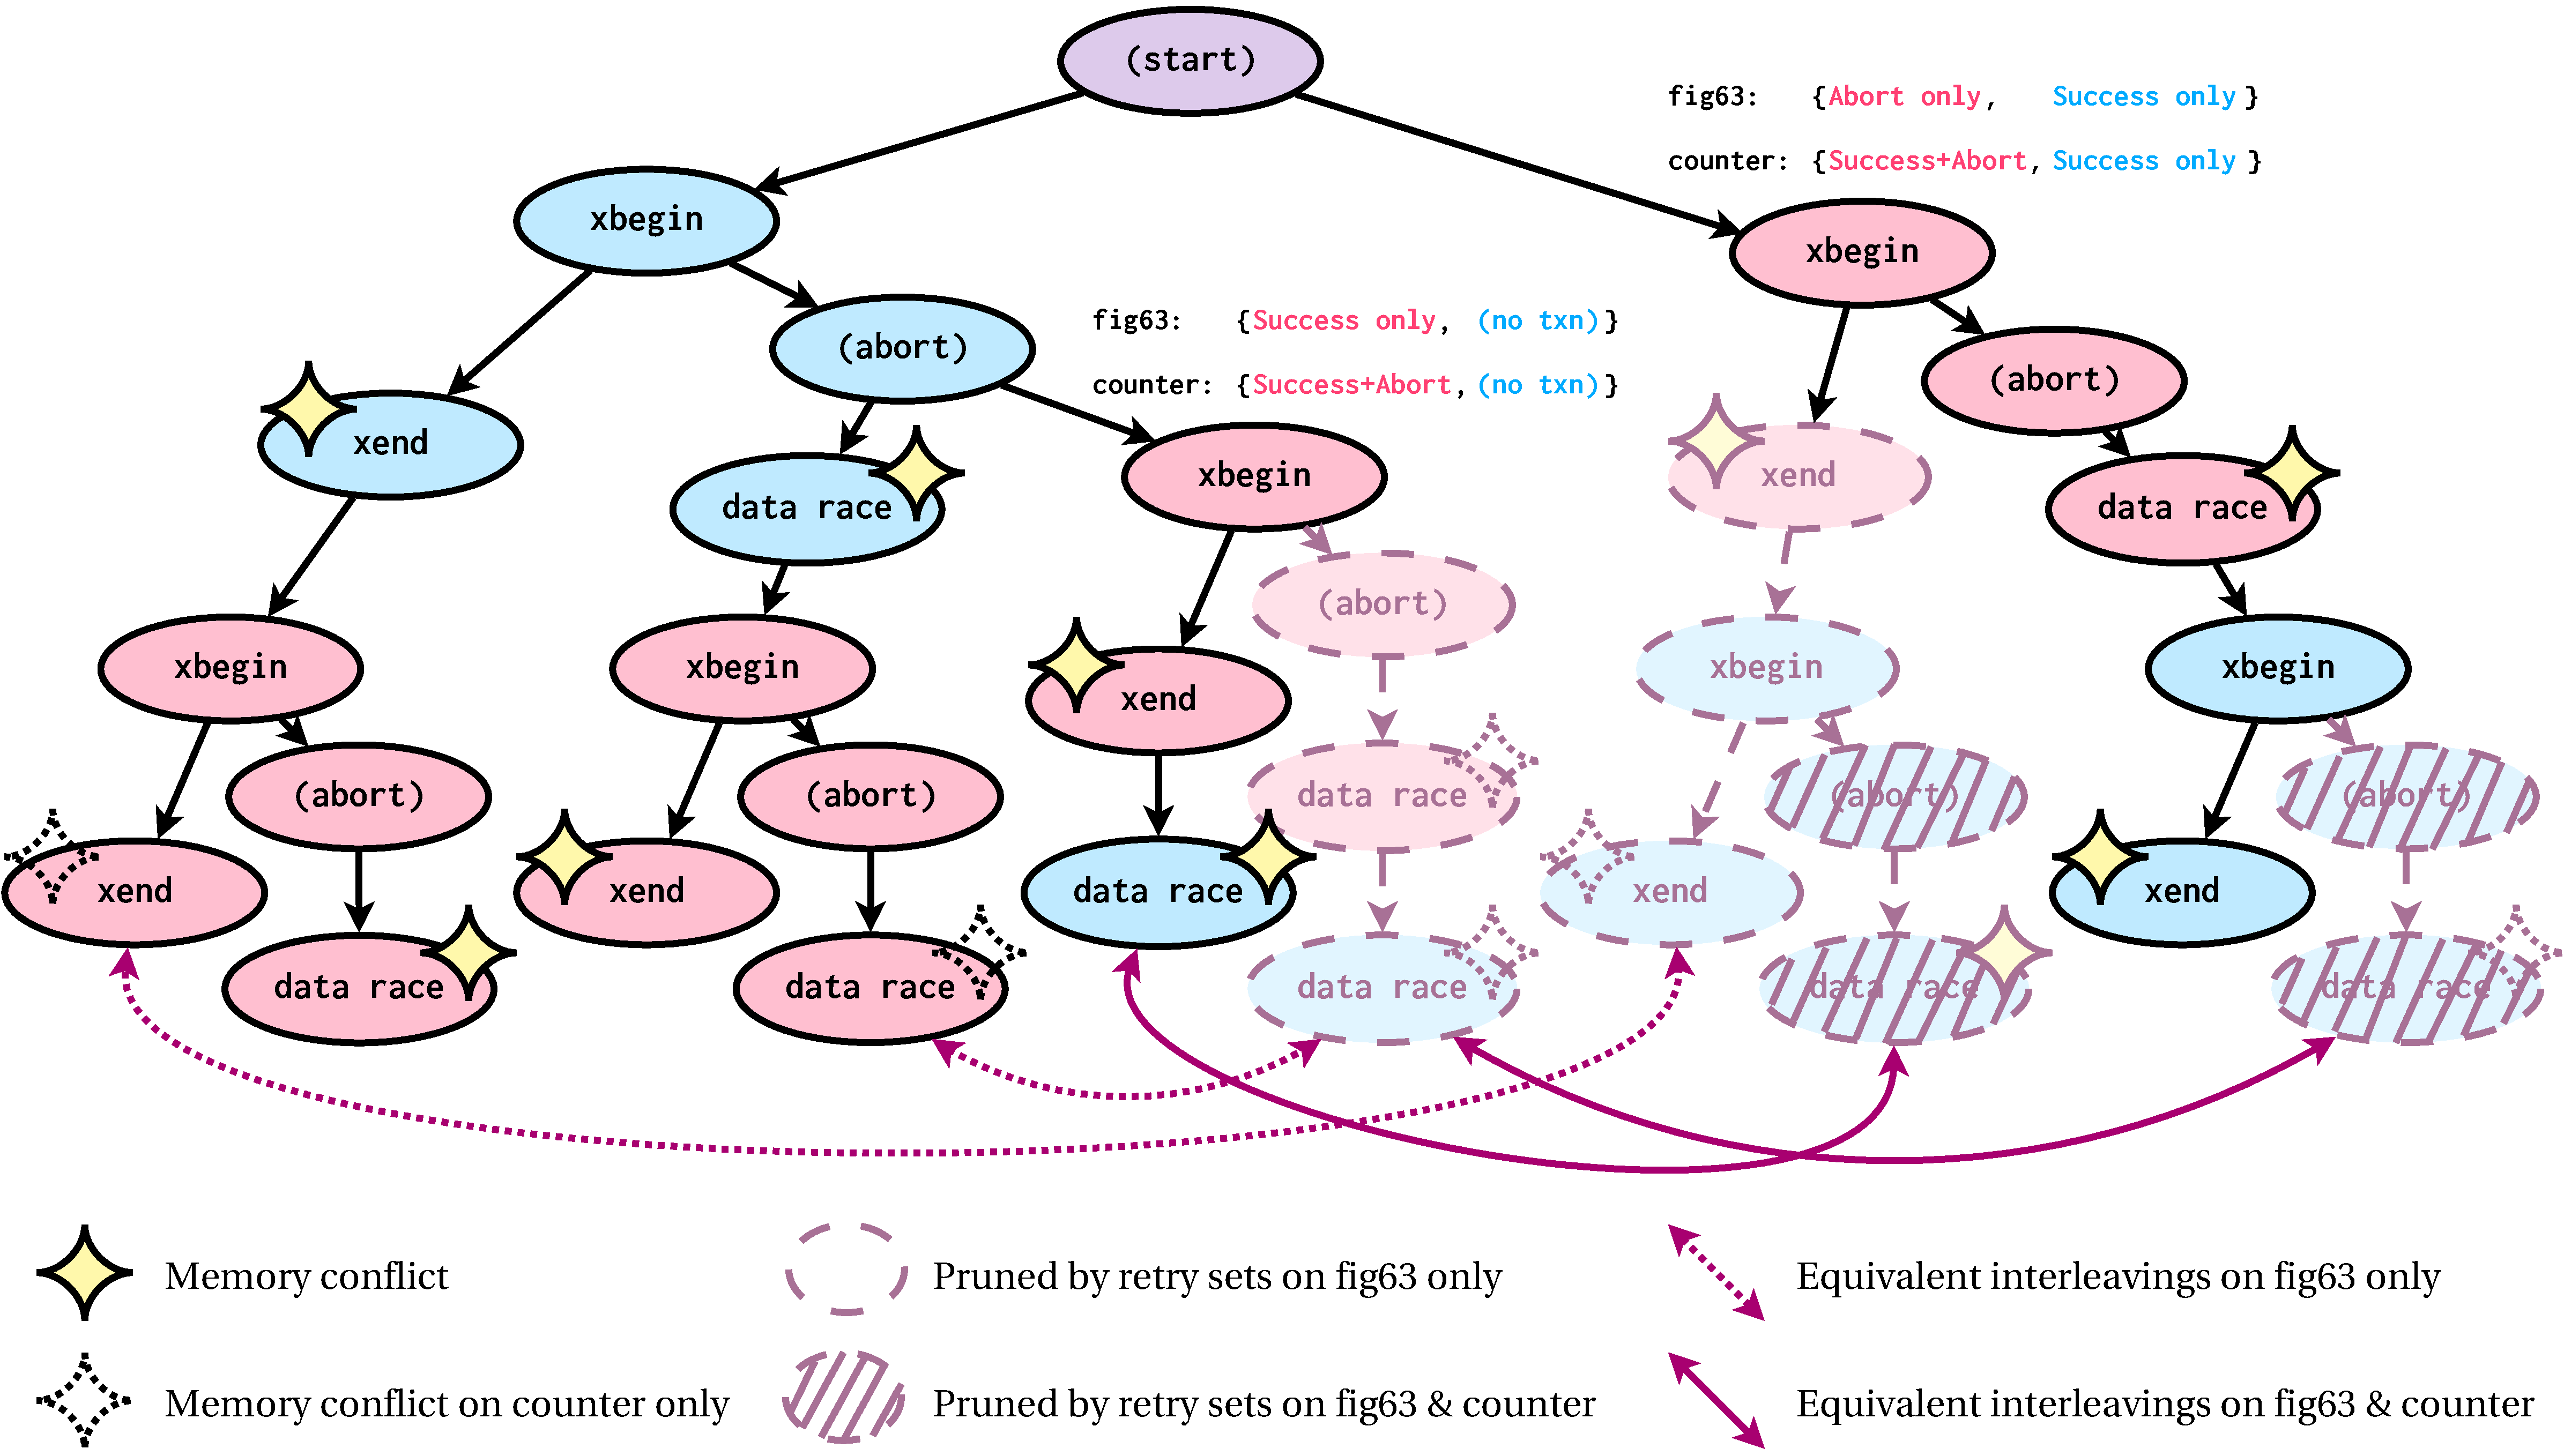
\includegraphics[width=\textwidth]{retry-sets.pdf}
	\end{center}
	\caption{Visualization of retry set state space reduction.
	On both {\tt counter}(2,1) and {\tt fig63}(2,1), baseline DPOR tests % oops
	all 10 interleavings pictured,
	with the middle 2 arising from the data-race preemption point within the abort path.
	%On {\tt counter}, all transitions marked as memory conflicts conflict with each other;
	%on {\tt fig63}, only pairs of one {\tt xend} and one {\tt data race} each conflict.
	With the reduction enabled,
	after the 4th and 6th branches
	(i.e., when preempting to reorder threads),
	Landslide activates the retry set
	indicated at the top of the next upcoming subtree,
	allowing it to identify and skip 2 redundant branches in {\tt counter}
	and 4 in {\tt fig63}.
	%to remember which parts of it to skip.
	}
	\label{fig:retry-reduction}
\end{figure}

Perhaps surprisingly, retry sets also provide reduction
even when transactional success and abort paths are fully conflicting,
(i.e., all tests besides {\tt fig63}).
With just synchronization preemption points (including {\tt \_xbegin()} and {\tt \_xend()}),
both the baseline and retry sets would explore exactly all 8 permutations of success and abort between two threads.
However, in the presence of data-race preemption points,
even for example on {\tt counter}(2,1)
(whose abort path is just 1 {\tt xadd} operation),
and whose optimal state space size should be 8 regardless of data-race preemption points),
baseline DPOR tests reorderings of one thread's transaction both with the other's failure path,
and with the other's data race therein%
\footnote{
Not pictured in Figure~\ref{fig:retry-reduction} is the symmetric subtree of branches 5-6 in the right half of the state space,
which would occur after branch 10, reordering the blue thread before the pink's data race.
Such would be equivalent to branches 2 and 4,
and is pruned by the normal sleep set algorithm (\sect{\ref{sec:landslide-sleepsets}}, {\tt equiv\_already\_explored()})
even in baseline DPOR, with no need for retry sets.
}.
Retry sets on the other hand identify and skip that equivalence
(technically speaking, retry set DPOR reorders with the data race first during depth-first search,
then skips generating a retry set for reordering the full abort path).

% --- counter-retry       2018-08-03 13:50:37.324021777 -0400
% +++ counter-baseline    2018-08-03 13:50:53.059021559 -0400
%  0--1@105c41 1-4@105c41 2-5@xbeg-delay 3-5@xbegin 4-5@xend 5-5@105c41 6-4@1001042 7-4@105c41 8-6@xbeg-delay 9-6@xbegin 10-6@xend 11-6@105c41 12-4@1001042 13-4@105c41 14-3@1028e9
% #[EXPLORE]       dbg #2/tid5 retry set: {TID6 (1,0), TID5 (1,0)}
% #[EXPLORE]       from #14/tid3, chose tid 6 (xabort injection), child of #9/tid6
%  0--1@105c41 1-4@105c41 2-5@xbeg-delay 3-5@xbegin 4-5@xend 5-5@105c41 6-4@1001042 7-4@105c41 8-6@xbeg-delay 9-6@xbegin 10-6@datarace-a 11-6@105c41 12-4@1001042 13-4@105c41 14-3@1028e9
% #[EXPLORE]       dbg #2/tid5 retry set: {TID6 (1,0), TID5 (1,0)}
% #[EXPLORE]       dbg #2/tid5 retry set: {TID6 (0,1), TID5 (1,0)}
% #[EXPLORE]       from #14/tid3, chose tid 5 (xabort injection), child of #3/tid5
%  0--1@105c41 1-4@105c41 2-5@xbeg-delay 3-5@xbegin 4-5@datarace-a 5-5@105c41 6-4@1001042 7-4@105c41 8-6@xbeg-delay 9-6@xbegin 10-6@xend 11-6@105c41 12-4@1001042 13-4@105c41 14-3@1028e9
% #[EXPLORE]       from #14/tid3, chose tid 6 (xabort injection), child of #9/tid6
%  0--1@105c41 1-4@105c41 2-5@xbeg-delay 3-5@xbegin 4-5@datarace-a 5-5@105c41 6-4@1001042 7-4@105c41 8-6@xbeg-delay 9-6@xbegin 10-6@datarace-a 11-6@105c41 12-4@1001042 13-4@105c41 14-3@1028e9
% #[EXPLORE]       from #14/tid3, chose tid 6, child of #4/tid5
%  0--1@105c41 1-4@105c41 2-5@xbeg-delay 3-5@xbegin 4-5@datarace-a 5-6@xbeg-delay 6-6@xbegin 7-6@xend 8-6@105c41 9-5@105c41 10-4@1001042 11-4@1001042 12-4@105c41 13-3@1028e9
% #[EXPLORE]       from #13/tid3, chose tid 6 (xabort injection), child of #6/tid6
%  0--1@105c41 1-4@105c41 2-5@xbeg-delay 3-5@xbegin 4-5@datarace-a 5-6@xbeg-delay 6-6@xbegin 7-6@datarace-a 8-6@105c41 9-5@105c41 10-4@1001042 11-4@1001042 12-4@105c41 13-3@1028e9
% #[EXPLORE]       from #13/tid3, chose tid 6, child of #2/tid5
% #[D-MAIL]        tt'ing abort set: {TID6 (1,0), TID5 (1,0)}
%  0--1@105c41 1-4@105c41 2-5@xbeg-delay 3-6@xbeg-delay 4-6@xbegin 5-6@xend 6-6@105c41 7-5@xbegin 8-5@xend 9-5@105c41 10-4@1001042 11-4@1001042 12-4@105c41 13-3@1028e9
% #[EXPLORE]       from #13/tid3, chose tid 6, child of #2/tid5
% #[D-MAIL]        tt'ing abort set: {TID6 (0,1), TID5 (1,0)}
% +0--1@105c41 1-4@105c41 2-5@xbeg-delay 3-6@xbeg-delay 4-6@xbegin 5-6@xend 6-6@105c41 7-5@xbegin 8-5@datarace-a 9-5@105c41 10-4@1001042 11-4@1001042 12-4@105c41 13-3@1028e9
%  0--1@105c41 1-4@105c41 2-5@xbeg-delay 3-6@xbeg-delay 4-6@xbegin 5-6@datarace-a 6-6@105c41 7-5@xbegin 8-5@xend 9-5@105c41 10-4@1001042 11-4@1001042 12-4@105c41 13-3@1028e9
% +0--1@105c41 1-4@105c41 2-5@xbeg-delay 3-6@xbeg-delay 4-6@xbegin 5-6@datarace-a 6-6@105c41 7-5@xbegin 8-5@datarace-a 9-5@105c41 10-4@1001042 11-4@1001042 12-4@105c41 13-3@1028e9

% --- fig-retry   2018-08-03 16:41:45.910879780 -0400
% +++ fig-baseline        2018-08-03 16:42:02.822879546 -0400
% @@ -16 +110 @@
%  7-5@xbegin 8-5@xend 9-5@105c41 10-6@105c41 11-4@105c41 12-6@105c41 13-4@105c41 14-6@1008178 15-6@xbegin 16-6@xend 17-6@105c41 18-3@1028e9
%  7-5@xbegin 8-5@xend 9-5@105c41 10-6@105c41 11-4@105c41 12-6@105c41 13-4@105c41 14-6@1008178 15-6@xbegin 16-6@datarace-a 17-6@datarace 18-6@105c41 19-3@1028e9
% #[EXPLORE]       dbg #6/tid5 retry set: {TID6 (0,1), TID5 (1,0)}
% #[EXPLORE]       from #19/tid3, chose tid 5 (xbegin failure injection), child of #7/tid5
%  7-5@xbegin 8-5@datarace-a 9-5@datarace 10-5@105c41 11-6@105c41 12-4@105c41 13-6@105c41 14-4@105c41 15-6@1008178 16-6@xbegin 17-6@xend 18-6@105c41 19-3@1028e9
% #[EXPLORE]       dbg #9/tid5 retry set: {TID6 (1,0), TID5 (1,1)}
% #[EXPLORE]       dbg #6/tid5 retry set: {TID6 (0,1), TID5 (1,0)}
% #[EXPLORE]       from #19/tid3, chose tid 6 (xbegin failure injection), child of #16/tid6
%  7-5@xbegin 8-5@datarace-a 9-5@datarace 10-5@105c41 11-6@105c41 12-4@105c41 13-6@105c41 14-4@105c41 15-6@1008178 16-6@xbegin 17-6@datarace-a 18-6@datarace 19-6@105c41 20-3@1028e9
% #[EXPLORE]       dbg #9/tid5 retry set: {TID6 (1,0), TID5 (1,1)}
% #[EXPLORE]       dbg #6/tid5 retry set: {TID6 (0,1), TID5 (1,0)}
% #[EXPLORE]       from #20/tid3, chose tid 6, child of #9/tid5
% #[D-MAIL]        tt'ing abort set: {TID6 (1,0), TID5 (1,1)}
%  7-5@xbegin 8-5@datarace-a 9-5@datarace 10-6@105c41 11-4@105c41 12-6@105c41 13-4@105c41 14-6@1008178 15-6@xbegin 16-6@xend 17-6@105c41 18-5@105c41 19-3@1028e9
% #[EXPLORE]       dbg #6/tid5 retry set: {TID6 (0,1), TID5 (1,0)}
% #[EXPLORE]       from #19/tid3, chose tid 6, child of #6/tid5
% #[D-MAIL]        tt'ing abort set: {TID6 (0,1), TID5 (1,0)}
% +7-5@xbegin 8-5@datarace-a 9-5@datarace 10-6@105c41 11-4@105c41 12-6@105c41 13-4@105c41 14-6@1008178 15-6@xbegin 16-6@datarace-a 17-6@datarace 18-6@105c41 19-5@105c41 20-3@1028e9
% +7-6@105c41 8-4@105c41 9-6@105c41 10-4@105c41 11-6@1008178 12-6@xbegin 13-6@xend 14-6@105c41 15-5@xbegin 16-5@xend 17-5@105c41 18-3@1028e9
% +7-6@105c41 8-4@105c41 9-6@105c41 10-4@105c41 11-6@1008178 12-6@xbegin 13-6@xend 14-6@105c41 15-5@xbegin 16-5@datarace-a 17-5@datarace 18-5@105c41 19-3@1028e9
%  7-6@105c41 8-4@105c41 9-6@105c41 10-4@105c41 11-6@1008178 12-6@xbegin 13-6@datarace-a 14-6@datarace 15-6@105c41 16-5@xbegin 17-5@xend 18-5@105c41 19-3@1028e9
% +7-6@105c41 8-4@105c41 9-6@105c41 10-4@105c41 11-6@1008178 12-6@xbegin 13-6@datarace-a 14-6@datarace 15-6@105c41 16-5@xbegin 17-5@datarace-a 18-5@datarace 19-5@105c41 20-3@1028e9


\subsubsection{STM (abort code) reduction}
\label{sec:tm-eval-stm}

Secondly, the state spaces could be reduced
simply by restricting the concurrency model
to only a subset of nondeterministic {\tt xbegin} outcomes possible under HTM.
Concretely speaking,
the {\tt -X -A -S} combination of Landslide options
suppresses retry aborts
(\sect{\ref{sec:txn-abort-codes}}),
which must be checked at every transactional preemption point,
replacing them with explicit and conflict aborts,
which Landslide injects only after identifying memory conflicts through DPOR
or encountering an {\tt xabort},
respectively,
ultimately simulating the semantics of STM rather than HTM.
This can allow for state space reduction %result in smaller state spaces compared to the baseline
when transactions happen to be non-conflicting,
but more impactfully,
conflict aborts can occur only {\em after} the other thread's conflicting access,
so between a pair of transactions
% only the first two during execution, not true for subsequent pairs, if they are in conflict with previous pairs at all
only the success, success and success, abort sequences need be tested;
abort, success and abort, abort may (in fact, must) be skipped.
The final column in Table~\ref{tab:tm-verifs} shows the result of STM semantics verification,
which always results in at least 2x reduction compared to the baseline,
although retry sets can make up some of the lost ground in some cases.

\subsubsection{Abstraction reduction}
\label{sec:tm-abstraction}

Visual inspection of the AVL tree and separate-chaining map implementations \cite{tm-benchmark-cmu},
after correcting the former's atomicity bug (Figure~\ref{fig:avlbug}),
reveals that every use of HTM followed exactly the same pattern:
running identical data structure logic in both the transactional and abort paths,
as though HTM were merely a mutual exclusion lock with fancy performance characteristics.
% this citation is a lil problematic
Prior work \cite{dbug-phdthesis} proposed {\em abstraction reduction},
in which the user identifies program components that can be separated by a well-understood API,
then tests each one against the API individually,
effectively turning multiplicative state space size factors into additive ones.

In this case, I split the lock-like HTM use
and the mutually-exclusive data structure code
into separate tests,
{\tt lock}, which checks that the use of HTM guarantees mutual exclusion,
and {\tt avl\_mutex}/{\tt map\_mutex},
which replace the open-coded HTM use with an already-trusted P2 mutex.
{\tt lock\_fast},
a bonus test,
checks the transactional lock's performance by asserting that
its internal logic won't trigger conflict aborts
even when the client's accesses are independent.
Figure~\ref{fig:htm-lock} shows their core logic.
Finally, I parameterized them over how the lock was implemented:
a real-world {\tt spinlock} implementation from \cite{spinlock-rtm-github},
{\tt spin\_fixed}, the same with the performance bug from \sect{\ref{sec:tm-eval-bugs}} fixed,
and {\tt mutex}, using Landslide-annotated P2 mutexes (as the AVL and map implementations do).

\begin{figure}[h]
	\begin{center}
	\begin{tabular}{p{0.47\textwidth}p{0.5\textwidth}}
		\begin{tabular}{l}
			\texttt{\ctype{static int} num\_in\_section = 0;} \\
			\texttt{\flow{for} (\ctype{int} i = \const{0}; i < \const{NITERS}; i++) \{} \\
			\texttt{~~~~\call{rtm\_spinlock\_acquire}(\&lock);} \\
			\texttt{~~~~num\_in\_section++;} \\
			\texttt{~~~~\flow{if} (!\call{\_xtest()})} \\
			\texttt{~~~~~~~~\call{thr\_yield}(\const{-1});} \\
			\texttt{~~~~\flow{assert}{}(num\_in\_section == \const{1}); } \\
			\texttt{~~~~num\_in\_section--;} \\
			\texttt{~~~~\call{rtm\_spinlock\_release}(\&lock);} \\
			\texttt{\}} \\
		\end{tabular}
		&
		\begin{tabular}{ll}
			\texttt{\flow{for} (\ctype{int} i = \const{0}; i < \const{NITERS}; i++) \{} \\
			\texttt{~~~~\call{rtm\_spinlock\_acquire}(\&lock);} \\
			\texttt{~~~~\flow{assert}{}(\call{\_xtest}());} \\
			\texttt{~~~~\call{rtm\_spinlock\_release}(\&lock);} \\
			\texttt{\}} \\
		\end{tabular}
		\\
		\\
		(a) {\tt lock}(), tests mutual exclusion.
		&
		(b) {\tt lock\_fast}(), tests for no spurious aborts.
	\end{tabular}
	\end{center}
	\caption{Abstraction reduction test cases.}
	\label{fig:htm-lock}
\end{figure}

Table~\ref{tab:tm-verifs2} shows the new resulting levels of verification
Landslide reached before the same 10-hour timeout.
Provided that one trusts the {\tt lock} tests correctly check the desired properties,
and that open-coding hadn't introduced any new bugs (such as Figure~\ref{fig:avlbug}'s),
the benefit is clear:
the data structure tests' state spaces become much more tractable,
%the data structure tests suddenly reach unprecedented thread/iteration counts with ease,
% 'so on' here includes free/re-malloc mem conflicts; see comment in avl_mutex.cpp
their state space growth now defined only by internal conflicts from tree rebalancing, map resizing, and so on.
In total,
summing the testing times of {\tt lock}({\tt mutex})$(K,N)$ and {\tt avl\_mutex}$(K,N)$
produces the same verification as {\tt avl\_fixed}$(K,N)$ far more cheaply.
Furthermore, {\tt lock}'s verification can be reused,
whereas {\tt avl\_fixed} and {\tt map\_basic} effectively duplicated the mutex verification between them.

\begin{table}[t]
	\begin{center}
		\footnotesize
		\begin{tabular}{cc}
		\begin{tabular}{cc||r|r}
			& & \multicolumn{2}{c}{\bf STM ({\tt -A -S})} \\
			& & \cpu{\bf cpu (s)} & \ints{\bf SS size} \\
			\bf test & \bf K,N  & \em (or \ETAdag{\bf \em est.})
			                      & \em (or \ETAdag{\bf \em est.}) \\
			\hline
			\hline
			{\tt lock}
			& 2,1 & \cpu{3.41} & \ints{4} \\
			({\tt spinlock})
			& 2,2 & \cpu{198.77} & \ints{1702} \\
			% if lock(spin_fixed) will time out on 2,3 and 3,2, this is guaranteed to aswell
			& 3,1 & \cpu{35.28} & \ints{246} \\
			\hline
			{\tt lock}
			& 2,1 & \cpu{3.55} & \ints{4} \\
			({\tt spin\_fixed})
			& 2,2 & \cpu{105.57} & \ints{998} \\
			& 2,3 & \ETAdag{33h 13m} & \ETAdag{321553} \\
			% [JOB 4] progress: 138911/321553 brs (43.200015%), ETA 23h 12m 50s (elapsed 9h 59m 48s)
			% total CPU time consumed: 10h 4s (36004577784 usecs) (core saturation: 12%)
			& 3,1 & \cpu{28.27} & \ints{186} \\
			& 3,2 & \ETAdag{13y 281d} & \ETAdag{1443676} \\
			% [JOB 4] progress: 169893/1443676 brs (11.768080%), ETA 13y 280d 17h 30m 54s (elapsed 9h 59m 48s)
			& 4,1 & \ETAdag{16h 26m} & \ETAdag{432628} \\ % was: 30408, 282084 pre mkrun
			% [JOB 4] progress: 286910/432628 brs (66.317896%), ETA 6h 26m 25s (elapsed 9h 59m 48s)
			% total CPU time consumed: 10h 4s (36004288982 usecs) (core saturation: 12%)
			\hline
			{\tt lock}
			& 2,1 & \cpu{3.44} & \ints{4}		\\
			({\tt mutex})
			& 2,2 & \cpu{16.83} & \ints{180}	\\
			& 2,3 & \cpu{405.21} & \ints{9372}	\\
			& 2,4 & \cpu{24999.68} & \ints{489480}	\\ % was: 15266 sec 384512 pre mkrun
			% total CPU time consumed: 6h 56m 39s (24999680839 usecs) (core saturation: 12%)
			& 3,1 & \cpu{15.00} & \ints{132}	\\
			%& 3,2 & \cpu{29432.87} & \ints{707086}	\\ % pre mkrun fix (let alone bottom1)
			& 3,2 & \ETAdag{26h 42m} & \ETAdag{1223955} \\
			% [JOB 2] progress: 714882/1223955 brs (58.407517%), ETA 16h 41m 58s (elapsed 9h 59m 55s)
			% total CPU time consumed: 10h 3s (36003621109 usecs) (core saturation: 12%)
			& 4,1 & \cpu{665.89} & \ints{15064}	\\
			\hline
			{\tt lock\_fast}
			& 2,1 & \cpu{3.25} & \ints{1}	\\
			({\tt spin\_fixed})
			& 9,9 & \cpu{4.61} & \ints{1}	\\
			\hline
			{\tt lock\_fast}
			& 2,1 & \cpu{3.19} & \ints{1}	\\
			({\tt mutex})
			& 9,9 & \cpu{4.62} & \ints{1}	\\
			\end{tabular}
			&
			\begin{tabular}{cc||r|r}
			& & \multicolumn{2}{c}{\bf Non-transactional} \\
			& & \cpu{\bf cpu (s)} & \ints{\bf SS size} \\
			\bf test & \bf K,N & \em (or \ETAdag{\bf \em ETA}) & \em (or \ETAdag{\bf \em est.}) \\
			\hline
			\hline
			{\tt avl\_mutex}
			& 2,1 & \cpu{3.48} & \ints{7} \\
			& 2,2 & \cpu{6.25} & \ints{85} \\
			& 2,3 & \cpu{24.69} & \ints{561} \\
			& 2,4 & \cpu{217.98} & \ints{4984} \\
			& 3,1 & \cpu{8.26} & \ints{129} \\
			& 3,2 & \cpu{1403.46} & \ints{30653} \\
			& 3,3 & \ETAdag{qqq} & \ETAdag{qqq} \\
			& 4,1 & \cpu{199.96} & \ints{4488} \\
			& 4,2 & \ETAdag{qqq} & \ETAdag{qqq} \\
			\cline{1-4}
			{\tt map\_mutex}
			& 2,1 & \cpu{39.81} & \ints{83} \\
			& 2,2 & \ETAdag{26h 21m} & \ETAdag{1085126} \\
			% [JOB 9] progress: 496530/1085126 brs (45.757812%), ETA 16h 21m 0s (elapsed 9h 59m 38s)
			% total CPU time consumed: 10h 19s (36019507965 usecs) (core saturation: 12%)
			& 3,1 & \ETAdag{173d 17h} & \ETAdag{12572187} \\
			% [JOB 9] progress: 496281/12572187 brs (3.947451%), ETA 173d 6h 38m 55s (elapsed 9h 59m 43s)
			% total CPU time consumed: 10h 20s (36020148608 usecs) (core saturation: 12%)
			\\
			\\
			\\
			\\
			\\
		\end{tabular}
		\\
		\\
		(a) Verifying HTM locks alone.
		&
		(b) Verifying the lock's client code.
		\end{tabular}
	\end{center}
	\caption{Continuation of Table~\ref{tab:tm-verifs},
		demonstrating abstraction reduction \cite{dbug-phdthesis}
		on the {\tt avl\_fixed} and {\tt map\_basic} tests
		by verifying HTM mutex implementations separately.
		Tested with STM semantics, as both lock implementations include a retry loop.}
	\label{tab:tm-verifs2}
\end{table}

Note two curiosities:
firstly,
the impact that fixing Figure~\ref{fig:spinlockbug}'s performance bug
(changing a read+write to a read only)
had on even the correctness tests:
{\tt lock}({\tt spin\_fixed})'s state spaces were reduced by nearly half compared to {\tt lock}({\tt spinlock}),
on account of DPOR no longer needing to reorder the (now) read-read access pairs.
Secondly, {\tt spinlock} and {\tt spin\_fixed} take longer to test per interleaving
%(CPU time divided by state space size)
than {\tt mutex}
% TODO recalc
(roughly 9 interleavings per second for the former, 22 for the latter),
because while {\tt mutex} abstracts away threads needing to wait their turn for the critical section
behind an API Landslide understands,
the spinlock's wait loop is open-coded, and Landslide must fall back on its costlier heuristic synchronization detection
(\sect{\ref{sec:landslide-blocking}}).
In this way (and also, of course, because {\tt mutex}'s state spaces are smaller overall),
{\tt mutex} can be seen in turn as a further abstraction reduction of {\tt spinlock}.

% commentary -- writing this test case well requires expert knowledge of noobs (of writing landslide friendly tests)
% - placing the asserts well, using sync_test_and_set and asserting on the result rather than having a separate read,
%   has an impact on the state space, as seen above
% - design of critical_section and how it uses xtest to yield only in failure path, and why that's justified

% other one to test -
% https://github.com/vamsikc/leveldb-tsx/blob/master/ext/xsync/include/scope.hpp

% "Although I skipped implementing it to begin with, the sheer size of this reduction also
% reflects on the numbers one might see betwee the original reduction in theorem so-and-so that lets us
% treat transactional success paths as mutually-exclusive (and, once started, abort-proof) to begin with"
% this sentence is a complete mess....

%%%%%%%%%%%%%%%%%%%%%%%%%%%%%%%%%%%%%%%%%%%%%%%%%%%%%%%%%%%%%%%%%%%%%%%%%%%%%%%%

\section{Discussion}

In this section I review some of the evaluation's results in a broader context,
list the current limitations of Landslide's implementation,
and discuss open problems for future work.

\subsubsection{Retry set optimality}

For all the reduction retry sets demonstrated in Table~\ref{tab:tm-verifs},
some inefficiencies remain in its strategy.
For example, it is not clear how to prune soundly
when three or more threads must be reorderd around one transactional preemption point,
or when a second pair of partially-independent transactions interleaves while an existing retry set is already active.
Accordingly, I implemented the optimization as conservatively as possible in these cases,
``saturating'' the retry sets to fall back to no pruning
({\tt update\_hax\_abort\_set()} and
{\tt update\_hax\_abandon\_abort\_set()}, respectively).

Likewise, the cases of {\tt htm2}(2,3) and (4,1),
in which retry sets achieved better reduction than STM mode,
show that the latter does not necessarily subsume the former,
and that combining the two could in theory achieve further reduction still.
However, {\tt xbegin} results other than {\tt \_XABORT\_RETRY}
may depend on the execution logic
(explicit aborts may be conditional on some change by a conflicting thread,
and conflict aborts cannot occur before their conflicting transaction to begin with%
\footnote{See {\tt 410user/progs/htm\_causality.c}; that was a fun realization to have
already halfway into implementing retry sets the wrong way at first.}%
),
so how to soundly prune either success paths or retry aborts
while other abort codes are in play
remains an open problem.

While
%the basic idea is
motivated by straightforward analogy to the known-sound sleep sets,
the intersection of retry sets with Landslide's other exploration features may cause unforeseen problems.
For now, its use is prohibited in conjunction with other state-space-affecting features
such as ICB (\sect{\ref{sec:landslide-icb}})
as well as multiple abort codes.
I personally believe retry set reduction to be sound under these restrictions,
having carefully scrutinized its behaviour
while constructing Figure~\ref{fig:retry-set-example}
and from inspecting state spaces arising from larger test parameters as well; %while implementing it;
nevertheless, this falls well short of formal proof, which I must leave to future work.

\subsubsection{STM reduction soundness}

In \sect{\ref{sec:tm-eval-stm}} I showed that state spaces could be reduced even further than with retry sets
by assuming an HTM interface which abstracts away {\tt \_XABORT\_RETRY} behind a loop.
However, suppressing retry aborts is not guaranteed to faithfully test all possible behaviours
observable under HTM.
As an example, note in Table~\ref{tab:tm-verifs}
how STM semantics reduced % oops
{\tt fig63}'s state space on all $(K,N)$ configurations to 1.
Because its transactional paths are all mutually independent,
DPOR identifies no need either to inject conflict aborts or to reorder threads.
However, this skips the slow-path consistency assertion completely.
If the programmer had intended it to run ``every so often'' at the whim of the timer interrupt,
applying this reduction would be unsound.
Also note the state space size of 4 for many (2,1) test configurations,
corresponding exactly to the aforementioned success, success and success, abort sequences
(times two ways to interleave the two threads).
Because of the scheduling dependency for conflict aborts,
Landslide cannot recognize the failure path's data races
without a third freely-reorderable iteration;
STM mode must be run with $K \times N \ge 3$ to meaningfully test conflicts between failure and success paths at all.
A user wishing to distinguish conflict aborts, retry aborts, and so on during testing
without glossing over any of HTM's peculiarities
could supply the {\tt -X -A} options without {\tt -S};
however, this will inevitably result in state spaces at least as large as the baseline.

On the other hand, some programs may clearly annotate their intention
for abort paths to be executed only in case of actual memory conflicts.
{\tt swap}, {\tt avl\_insert}, and {\tt map\_basic} abstract their {\tt \_xbegin()} calls
behind an interface which can be implemented either with or without retry loops,
while {\tt lock}({\tt spinlock}) and {\tt lock}({\tt mutex}) implement the retry loop directly.
In these cases, the user can assure herself of STM reduction's soundness by visual inspection.
In fact, Landslide's current implementation gets stuck in infinitely deep interleavings
whenever it encounters a retry loop
% not actually sure why, as it should be around-a-pp and not on the 1st branch...
(bypassing even its heuristic infinite loop detection),
so for now the user must inspect the test case to determine which testing mode to use.
Future work could automatically identify a program's retry loops
and give up on {\tt \_XABORT\_RETRY} by switching to STM mode on-the-fly,
much like Landslide's heuristic synchronization detection does for yield loops (\sect{\ref{sec:landslide-blocking}}).

\subsubsection{Nested transactions}
\label{sec:tm-warpzone-nested}

Whenever {\tt \_xbegin()} is called with a transaction already active, or {\tt \_xend()} while not,
Landslide's current implementation immediately stops and reports a bug.
However, just as concurrent programs often hold multiple locks simultaneously,
one may wish to conduct multiple transactional routines simultaneously,
especially as they may be abstracted across different code modules as a project grows in scale.
Recent work \cite{hybrid-htm-stm,relaxed-transactions-popl} has developed
both implementations and formal semantics for executing nested transactions,
so future work should extend the verification concurrency model to permit such programs.
For now, the best Landslide can offer is to check the transactional components and their client code
separately against their APIs
with abstraction reduction (\sect{\ref{sec:tm-abstraction}}),
then check the rest of the program with (for example) traditional mutexes that can nest safely.

\subsubsection{Relaxed memory orderings}
\label{sec:tm-warpzone-relaxed}

Section~\ref{sec:tm-design}'s formalization of thread interleavings does not account for read/write reorderings
possible on relaxed consistency architectures \cite{memory-consistency-models}.
In fact,
even after \cite{tm-benchmark-cmu}'s proposed fix to the atomicity protocol in Figure~\ref{fig:htm-fixed},
it is still incorrect on Total Store Order (TSO) architectures such as x86,
let alone on weaker memory models.
Despite stores being totally-ordered, x86 may still reorder stores after subsequent loads
\cite{sully-thesis}.
Accordingly, an execution of lines $8,9a,9b,9c$
may be locally visible to another thread as $9a,8,9b,9c$,
and hence an apparent interleaving of
\[
        \tiat{1},\tjat{1-5},\tiat{7},\underline{\tiat{9a}},\tkat{1-5},\underline{\tiat{8}},\tiat{9b-B}
\]
is possible
(reordered accesses underlined for emphasis).
An acquire barrier is needed between lines 8 and 9 to solve this problem on TSO \cite{tsx-need-barrier}
(on x86, either {\tt mfence} or {\tt xchg}/{\tt xadd}).
% gcc generates the latter for its __sync_lock_test_and_set intrinsic
Recent work \cite{relaxed-transactions-pldi} also demonstrated unsoundness
in a similar lock elision implementation on ARMv8 (PSO),
in which the transactional path reads the lock's internal state directly
rather than using a separate flag.
In Figure~\ref{fig:htm-fixed}, a release barrier before line A is also necessary under PSO.
% On Partial Store Order (PSO) architectures,
% %even more barriers may be necessary.
% a release barrier is necessary before line A as well.
% Recent work \cite{relaxed-transactions-pldi} also discovered similar unsoundness
% in lock elision \cite{speculative-lock-elision}
% on ARMv8 (PSO).
% Recent work \cite{relaxed-transactions-pldi} also discovered similar unsoundness

Because Landslide's concurrency model includes only instruction-level thread nondeterminism,
not per-CPU memory buffer reorderings,
its current HTM implementation cannot find this bug.
In fact, it erroneously verifies the corresponding test {\tt htm2}(3,1)
%% sigbovik version, probably pre-thrlib-function and definitely pre-dpor-preferred-tid and pre-trusted-join
% in 3 CPU-hours,
% with 467730 distinct interleavings in total,
in 40 CPU-seconds,
with 774 interleavings in total,
none of which include the above-listed sequence.
Recent work has extended DPOR to support TSO and PSO memory nondeterminism \cite{tsopso},
as well as proposed formal execution semantics for HTM on these architectures
\cite{relaxed-transactions-popl,relaxed-transactions-pldi};
if both of these advances were incorporated into Landslide's concurrency model,
it could find or verify the absence of such bugs.
Visual inspection of \cite{tm-benchmark-cmu}'s HTM data structures found no barriers used in this implementation pattern;
I would urge any reader interested in using those to add them in by hand first.
The test case {\tt lock}({\tt mutex}) ({\tt 410user/progs/htm\_mutex.c} in the repository)
provides an example of how to use compiler intrinsics to emit the necessary barriers.
